\documentclass[a4paper]{book}
\usepackage{geometry}
\usepackage{fontspec}
%\setmainfont[Ligatures=TeX]{DejaVu Sans}
\setmonofont{DejaVu Sans Mono}
\defaultfontfeatures{Ligatures=TeX}
\usepackage{polyglossia}
\setmainlanguage{spanish}

\usepackage{graphicx}
\graphicspath{{imgs/}}

\usepackage{url}
%\usepackage{hyperref}

\usepackage{minted}
\newminted{jlcon}{fontsize=\small}
\newminted{julia}{fontsize=\small}
\newmint{jlcon}{fontsize=\small}
\newmintinline{text}{breaklines=true, breakafter=()\[\]\{\}\,\.+-*/}
\newcommand{\code}{\textinline}
% Remove red boxes
\makeatletter
\expandafter\def\csname PYGdefault@tok@err\endcsname{\def\PYGdefault@bc##1{{\strut ##1}}}
\makeatother

%\usepackage{titlesec}
%\titleformat{\chapter}{\normalfont\huge}{\thechapter.}{20pt}{\huge\it}

\begin{document}
\chapter{Introducción}

\section{¿Por qué \emph{Julia}?}

Los lenguajes de programación dinámicos son una herramienta esencial en muchas profesiones científicas, que a menudo requieren realizar cálculos complejos en un corto plazo de tiempo; cálculos que además suponen un problema nuevo en cada ocasión, en el que los algoritmos a utilizar suelen basarse en trabajos anteriores, pero siempre necesitan ciertos retoques o extensiones.

La utilidad y popularidad de los distintos lenguajes existentes, y de las herramientas de software que los implementan, dependen de varios factores, y en particular del campo de aplicación y el contexto institucional. Tres de los más imporantes son R, Matlab y Python.

R es principalmente una herramienta para cálculos estadísticos, aunque también es posible utilizarlo para muchos otros propósitos. Se trata de una implementación a modo de software libre del lenguaje utilizado por el programa S-PLUS, con una comunidad de usuarios y desarrolladores espectacularmente activa, que ha extendido su potencia y funcionalidades a casi cualquier tipo de tratamiento de datos. En consecuencia, R es la opción más usada en la ciencia estadística, especialmente en el entorno académico (en ciertos sectores industriales tiene más presencia el programa y el lenguaje de SAS, propiedad de la compañía privada del mismo nombre).

Matlab es una de las soluciones más empleadas para la computación numérica en ciencias físicas e ingeniería, tanto por la industria como por la academia, gracias a la potencia de sus utilidades gráficas, numerosas \emph{toolboxes}, y un excelente entorno de desarrollo. Al contrario que R, se trata de un software cerrado y privado; existe también una implementación libre de Matlab (GNU Octave), que podría compararse con el caso de R respecto a S-PLUS, pero en este caso la herramienta libre no goza de tanta popularidad.

Python, por su lado, es un lenguaje de programación genérico, implementado en forma de software libre, que tiene la comunidad de usuarios más entusiasta y numerosa de todos los lenguajes citados. El campo de aplicación de Python va en realidad mucho más allá del científico, siendo un lenguaje que sirve para prácticamente cualquier tipo de operación informática. Pero existen varios módulos de Python recogidos en el paquete SciPy, específicamente dedicados a la computación numérica, que también se presentan como una alternativa libre a Matlab.

En este contexto, el Massachusets Institute of Technology (MIT) publicó en 2012 Julia, otro lenguaje dinámico para computación científica, bajo la licencia del MIT para software libre. A la vista del tipo de funciones y operaciones que ofrece, podría parecer que Julia intenta reinventar la rueda, aunque sus autores son plenamente conocedores del estado de la ciencia en lenguajes de programación. De hecho, la documentación oficial parece especialmente dirigida a programadores que ya conocen otros lenguajes, y en particular los tres mencionados. Según las propias declaraciones de los creadores de Julia,%
\footnote{%
\url{http://julialang.org/blog/2012/02/why-we-created-julia/}%
}
su finalidad es combinar lo mejor de cada uno de esos (y otros) lenguajes, y salvar el mayor obstáculo común de todos ellos: la velocidad para cálculos complejos y tratamiento de ficheros y bases de datos muy voluminosas.

El \emph{leit motiv} de Julia es principalmente su velocidad, comparable a la de programas compilados en C, sin dejar de ser un lenguaje plenamente dinámico y que permita trabajar con el paradigma del \emph{read-eval-print loop}. Esto hace que, incluso en su fase inicial de desarrollo, y con las carencias propias de la misma (pocos editores de código e interfaces para el desarrollo de programas, utilidades para depuración limitadas, etc.), Julia tenga un nicho de aplicación muy atractivo: la ejecución de operaciones conceptualmente sencillas, como algoritmos iterativos o rutinas masivas de lectura y escritura de dispositivos y archivos, que en lenguajes de bajo nivel pueden ser muy eficientes, pero a la hora de ejecutarlas en alguno de los lenguajes antes mencionados puedan consumir hasta horas de trabajo de la máquina. Con poco esfuerzo de programación, una hora de procesamiento en Matlab puede traducirse en unos pocos segundos de Julia.


\section{Primeros pasos}

\subsection{Instalación y uso básico de Julia}

Explicar los primeros pasos para usar un lenguaje de programación es algo delicado y difícil. Es habitual comenzar con ejercicios triviales como el del ``Hola mundo'', pero esos ejemplos no resultan muy estimulantes, ni dan tampoco una idea clara de cómo es el lenguaje. El extremo opuesto es comenzar con un fragmento de código para una aplicación relativamente compleja, que contenga buena parte de las características principales que se quieren explicar, e ir desgranándolas poco a poco, asumiendo que la mayor parte del programa será incomprensible para el lector hasta que haya avanzado bastante. Lo cierto es que esa es una aproximación más cercana al modo en el que la mayoría acaba haciendo frente a cualquier lenguaje en la ``vida real'', aunque también puede ser frustrante. Así que buscando un punto de compromiso, en esta sección se partirá de ejemplos prácticos pero sencillos, que se puedan entender por entero aunque los conceptos incluidos no se expliquen en detalle hasta secciones posteriores.

Ahora bien, antes de poner en práctica cualquier ejemplo, es necesario tener instaladas las herramientas que permiten usar el lenguaje de programación. El software básico para usar Julia está disponible en su página oficial (\url{http://julialang.org/downloads}), en forma de código fuente así como en binarios preparados para instalar en Windows, Mac OS X, y algunas distribuciones de Linux (por lo menos Ubuntu). Desde esa página se pueden encontrar también enlaces con explicaciones detalladas sobre cómo instalar y ejecutar Julia, que son específicas para cada sistema, y por lo tanto no desarrollaremos aquí.

Por defecto, al ejecutar Julia se abre el ``intérprete'' de comandos para trabajar de forma interactiva, que es el modo de uso de Julia más útil para aprender y hacer pruebas sencillas. Por otro lado, para ejecutar rutinas más complejas, y siempre que se quiera obtener resultados reproducibles, es recomendable escribir las instrucciones en un archivo de código, y luego ejecutarlo en Julia. Los entornos de desarrollo integrados, ``IDE'' en inglés, suelen tener editores de código que permiten combinar ambas tareas ---escribir instrucciones en un archivo de código y ejecutarlas--- desde la misma interfaz, lo cual facilita el trabajo del programador. (Véase más abajo sobre algunos IDE para Julia.)

Veamos ahora un ejemplo práctico de ambas formas de uso, con un programa sencillo para calcular el día de la semana en el que cae cualquier fecha del calendario Gregoriano, usando el algoritmo de Gauss tal como está publicado por Bernt Schwerdtfeger.%
\footnote{%
\url{http://berndt-schwerdtfeger.de/cal/cal.pdf}%
} Se trata de un algoritmo simple, que podría traducirse a Julia mediante el siguiente código: 

\begin{juliacode}
function gauss_diasemana(d, m, y)
# d, m, y son los números del día, mes y año, respectivamente
# La función devuelve una cadena de texto con el día de la semana
  # Enero y febrero (m=1, m=2) se tratan como el año anterior
  # en torno a los años bisiestos
  if m < 3
    y = y - 1
  end
  # Dividir el año entre centenas (c) y el resto (g)
  c = div(y, 100)
  g = mod(y, 100)
  # Definir e y f en función del mes (de 1 a 12) y el siglo
  # (en ciclos de 400 años --- 4 siglos)
  earray = [0,3,2,5,0,3,5,1,4,6,2,4]
  farray = [0,5,3,1]
  e = earray[m]
  f = farray[mod(c,4)+1]
  # Seleccionar el día de la semana en función del cálculo de Gauss
  warray = ["domingo","lunes","martes","miércoles","jueves","viernes","sábado"]
  w = mod(d + e + f + g + div(g, 4), 7)
  return(warray[w+1])
end
\end{juliacode}

Supongamos que ese código está guardado en un archivo llamado \code{calc_diasemana.jl} (el nombre del archivo es arbitrario, y puede ser cualquier nombre aceptado por el sistema operativo). El programa consiste en una sola función con 3 argumentos (los números del día, el mes y el año), basada en unas pocas divisiones enteras (definidas en la función \code{div}) y el cálculo de ``restos'' de dichas divisiones (\code{mod}),%
\footnote{%
Existen dos funciones para el resto de una división: \code{mod} y \code{rem}, que funcionan de forma distinta cuando alguno de los dos operandos es negativo. Para el caso que nos ocupa esa diferencia no es relevante.%
}
más la selección de unos valores a partir de los resultados intermedios y unas listas predefinidas.

Este programa se puede ejecutar de forma interactiva, usando la función \code{include} en el intérprete de Julia. Esto es lo que se debería ver en pantalla (el texto \code{julia>} al comienzo de la primera línea solo marca el punto de inserción del código; no es parte del código, y puede variar entre sistemas):

\begin{jlconcode}
julia> include("calc_diasemana.jl")
calc_diasemana (generic function with 1 method)
\end{jlconcode}

El resultado es algo decepcionante, porque lo único que se ha hecho es definir una función, que por sí misma no da ningún resultado. Por otro lado, lo más probable es que al introducir esa línea sin más ni siquiera se obtenga ese resultado, sino un error debido a que no se encuentra el archivo de código.%
\footnote{%
Ref. a sección con información sobre LOAD\_PATH y require()%
}
Para asegurarse de que Julia encuentra el archivo,
hay varias alternativas:

\begin{enumerate}
  \item Copiar el archivo de código \code{calc_diasemana.jl} al directorio de trabajo de Julia. La ruta de ese directorio se puede obtener con la función \code{pwd()} --- sin ningún argumento---.
  \item Cambiar el directorio de trabajo al lugar que contiene el archivo. El cambio de directorio se hace con la función \code{cd}, que recibe un solo argumento: el nombre del directorio destino. Este se puede definir literalmente como un texto entre comillas dobles, o ser una variable que contiene dicho texto. En sistemas operativos con entornos gráficos, puede ser práctico copiar el nombre del directorio desde el gestor de archivos al ``portapapeles'', y utilizarlo directamente en Julia con la función \code{clipboard}; es decir, introduciendo la expresión \code{cd(clipboard())}.%
  \footnote{%
  Esta solución es particularmente recomendable en Windows, donde los directorios de una ruta suelen presentarse divididos por ``barras invertidas''. Por ejemplo, el directorio de trabajo podría ser \code{C:\julia}. Pero la expresión \code{cd("C:\julia")} no daría el resultado esperado, porque la barra invertida se interpreta como inicio de una ``secuencia de escape'' para caracteres no imprimibles. Para que funcionase, habría que escribir \code{cd("C:/julia")} o \code{cd("C:\\julia")}. La función \code{clipboard} ahorra este tipo de problemas.%
  }
  \item Introducir la ruta completa del archivo de código en la llamada a \code{include}. Esta se puede escribir literalmente, o si el directorio que contiene el archivo está definido en una variable (supongamos que esta variable se llama \code{dir_include}, la ruta se puede componer con la función \code{joinpath}. Es decir, la expresión anterior sería \code{include(joinpath(dir_include, "calc_diasemana.jl"))}. También en este caso se podría utilizar \code{clipboard} para identificar el directorio destino a través del portapapeles.
\end{enumerate}

Una vez se ha conseguido cargar el archivo que define la función, esta ya se puede usar para obtener un resultado de verdad. Por ejemplo, para conocer en qué día de la semana cayó el San Valentín de 2012:

\begin{jlconcode}
julia> gauss_diasemana(14, 2, 2013)
"jueves"
\end{jlconcode}

Lo que se hace ``en un día cualquiera'' usando Julia es esencialmente este modelo de rutina, con funciones más complicadas y muchas más operaciones interactivas, explorando resultados, corrigiendo argumentos y repitiendo operaciones, claro está.


\subsection{Obtener ayuda}
Ayuda: help, documentación...


\subsection{Reglas sintácticas}

La sintaxis de los lenguajes de programación implica una multitud de reglas, la mayoría de las cuales en realidad no es necesario explicar, ya que son reglas de escritura lógicas e intuitivas, o se desprenden directamente de la lectura de ejemplos. Sin embargo, hay unos pocos detalles que pueden resultar menos claros y conviene mencionar.

Uno de estos detalles es el tipo de nombres permitidos para las variables y funciones. Las reglas son básicamente las habituales: pueden estar formados por cualquier combinación de letras y números, más guiones bajos, exceptuando nombres que comiencen por números y las palabras clave del lenguaje (como \code{for}, \code{if}, \code{end}, etc.). Además, también se admiten nombres con caracteres Unicode más allá del ASCII básico (letras acentuadas, griegas, etc.), así como el signo de exclamación (\code{!}) en posición no inicial, aunque conviene usarlos con mesura: emplear caracteres extendidos aumenta el riesgo de problemas de portabilidad de los programas, y la exclamación se suele resevar para el nombre de cierto tipo de funciones (las que modifican sus argumentos de entrada).

Hay seis constantes predefinidas que se pueden sobreescribir, pero conviene evitarlo (si se han usado antes en la sesión de Julia, aparecerá una advertencia al asignarles cualquier valor). Cuatro de ellas tienen dos nombres (tres con letras griegas), lo cual da más margen para reutilizar sus nombres:

\begin{itemize}
  \item \code{pi}, \code{$\pi$}: el número pi.
  \item \code{e}, \code{eu}: el número de Euler
  \item \code{eulergamma}, \code{$\gamma$}: la constante de Euler-Mascheroni.
  \item \code{golden}, \code{$\Phi$}: la proporción áurea.
  \item \code{catalan}: la constante de Catalan.
  \item \code{im}: la unidad imaginaria.
\end{itemize}

Los espacios entre nombres de variables, funciones, etc. son normalmente irrelevantes: siempre que haya algun símbolo delimitador (operadores matemáticos, signos de puntuación, paréntesis\ldots) pueden usarse uno, varios o ningún espacio entre ellos, o al principio de la línea. El uso de los espacio responde más a una cuestión de estilo que a la sintaxis. Por ejemplo, los distintos bloques de código (funciones, bucles, etc.) suelen sangrarse con un número de espacios en función del nivel de anidamiento (véase la función \code{gauss_diasemana} y el \code{if} anidado en ella), pero esto se hace para mejorar la legibilidad, no por necesidad (al contrario que en Python). Hay, sin embargo, dos excepciones.

Una de ellas es el paréntesis inicial de la llamada a ``macros''. A nivel de usuario una macro no resulta muy distinta a una función cualquiera, salvo en que el nombre empieza por la arroba (\code{@}), y en este detalle: el paréntesis ha de seguir al nombre de las macros sin ningún espacio intermedio (esta restricción no aplica a las funciones). Por ejemplo, para la macro \code{@printf} (usada para presentar valores en cadenas de texto con un formato específico):

\begin{jlconcode}
julia> # Correcto:
julia> @printf("El numero pi es %.4f", pi)
El numero pi es 3.1416
julia> # ¡Mal!
julia> @printf ("El numero pi es %.4f", pi)
ERROR: first or second argument must be a format string
\end{jlconcode}

Por otra parte, los argumentos de las macros pueden escribirse sin
paréntesis y separados por espacios, sin comas:

\begin{jlconcode}
julia> # Esto también vale:
julia> @printf "El numero pi es %.4f" pi
El numero pi es 3.1416
\end{jlconcode}

La otra excepción es la premultiplicación de variables por números literales. Como ya se ha dicho, el nombre de una variable no puede comenzar por un número, pero sí se puede \emph{añadir} un número ante el nombre de una variable, lo cual funciona como si esa variable se multiplicara por ese valor (como se hace muchas veces al escribir fórmulas textualmente). Por ejemplo:

\begin{jlconcode}
julia> 2pi # Equivale a 2*pi
6.283185307179586
\end{jlconcode}

Otro detalle importante es el uso del punto para distinguir números enteros y decimales. Para Julia el número \code{1} no es el mismo que \code{1.0}, aunque simbolicen el mismo valor. El primero es un número entero, cuya representación en la memoria del ordenador no es compatible con la de los números decimales, y para mayor eficiencia Julia usa procedimientos distintos para operar con cada tipo de número. En la mayoría de los casos el usuario puede pasar por alto esta distinción, ya que el procesador se encarga de hacer automáticamente las conversiones necesarias (normalmente transformando los números enteros a decimales). Sin embargo, en secciones posteriores, en particular al hablar de los \emph{arrays}, se verá que a veces hay que tener cuidado con estos detalles. Para definir un número explícitamente como decimal basta con incluir el punto; si su valor es entero no hace falta incluir los ceros a la derecha.

\begin{jlconcode}
julia> # Los enteros no son "iguales" a los decimales, aunque valen lo mismo
julia> 1 == 1.0
true
julia> isequal(1, 1.0)
false
julia> # Comprobar formas equivalentes de escribir números decimales
julia> isequal(1., 1.0)
true
julia> isequal(0.1, .1)
true
\end{jlconcode}

Finalmente, cabe mencionar el uso opcional del punto y coma (\code{;}) al final de las expresiones. Normalmente cada expresión de Julia se termina con un salto de línea, pero puede usarse un punto y coma en su lugar, lo cual tiene dos efectos. Por un lado, es posible añadir otra expresión tras el punto y coma en la misma línea. Por ejemplo:

\begin{jlconcode}
julia> a = 1; b = 2
\end{jlconcode}

Por otro lado, si se está trabajando en modo interactivo y no se añade ninguna otra expresión tras el punto y coma antes del salto de línea, no se presenta ningún resultado en pantalla. Este efecto no siempre es apreciable, ya que el procesador de Julia es por sí mismo bastante parco a la hora de presentar resultados. De hecho, \emph{nunca} presenta los resultados de las expresiones contenidas dentro de un bloque de código, independientemente de si llevan o no punto y coma al final.

En ocasiones esta última regla puede parecer confusa. Por ejemplo, considérese el siguiente bloque de código (delimitado por \code{begin} y \code{end} para forzar el agrupamiento de todas las líneas en un bloque):

\begin{juliacode}
begin
  x = 1
  y = 2
  z = 3
end
\end{juliacode}

Si se prueba a escribir y ejecutar el bloque en modo interactivo, se verá en pantalla el resultado de la última línea (\code{3}), pero no el de las demás. Sin embargo esto no tiene nada que ver con el hecho de que esa (o las otras líneas) lleven o no punto y coma. De hecho, ocurriría lo mismo si se añade el punto y coma a la tercera línea o cualquiera de las demás.

¿Por qué aparece entonces el \code{3} en pantalla? La respuesta es que el bloque delimitado por \code{begin}/\code{end} es también una expresión de Julia (una expresión compuesta), cuyo resultado es el de la última línea del código que contiene. Lo que se muestra en pantalla es por tanto el resultado del bloque completo. La prueba es que si se añade el punto y coma al final del mismo, tras la palabra \code{end}, ya no se verá nada en pantalla.

Algo semejante ocurre al cargar un fichero de código con la función \code{include}. Esta función también devuelve un resultado, que es el de la última línea del archivo, y se verá reproducido en pantalla salvo que se añada el punto y coma en la llamada a \code{include}.

\subsection{Complementos principales}

La distribución básica de Julia es realmente ``básica'', y carece de bastantes utilidades que son consideradas como muy importantes, incluso fundamentales, por la mayoría de los potenciales usuarios de un lenguaje de ese tipo, como representaciones gráficas de datos, editor de código, ayudas para la depuración de rutinas (\emph{debugging}), etc.

Esta limitación está cubierta por el desarrollo coordinado (aunque independiente) de cientos de ``paquetes'' que contienen dichas utilidades. Como el propio proyecto Julia, todos los paquetes oficiales están publicados con el sistema de \url{http://git-scm.com/}{Git}. Julia mantiene un catálogo online de los paquetes oficiales, cuya lista se puede consultar con la expresión \code{Pkg.available()}.

Su instalación y desinstalación se controla desde dentro de Julia, mediante las funciones \code{Pkg.add} y \code{Pkg.rm}, respectivamente, que toman como argumento el nombre del paquete a instalar o desinstalar. Estas operaciones consisten esencialmente en ``clonar'' el paquete publicado en un lugar determinado del sistema, o borrarlo de ese sitio (definido en la variable \code{JULIA_PKGDIR} si existe, o por defecto en el directorio designado por la función \code{Pkg.dir}). Por ejemplo, el proceso para instalar el paquete \code{Winston} (el más básico para representaciones gráficas) podría ser como sigue:

\begin{jlconcode}
julia> # Consultar si está instalado (en cuyo caso no hace falta instalarlo)
julia> Pkg.installed("Winston")

julia> # Si devuelve "nothing" (no está instalado):
julia> Pkg.add("Winston")
\end{jlconcode}

Esta operación solo hay que hacerla una vez (actualizaciones aparte). Sin embargo, tener el paquete instalado no basta para poder usarlo. Para esto último hay que cargarlo explícitamente en cada sesión de trabajo, con la instrucción \code{using}:

\begin{jlconcode}
julia> using Winston
\end{jlconcode}

A continuación se presenta una lista de algunos de los paquetes que pueden ser fundamentales para la mayoría de usuarios:

\begin{itemize}
  \item Gráficos: \code{Winston} (el paquete más básico), \code{Gadfly} (semejante al ggplot2 de R), \code{PyPlot} basado en Matplotlib, depende de tener instalada esa librería de Python.
  \item Salvar y leer variables generadas entre sesiones de Julia: \code{HDF5}.
  \item Depuración de funciones (básico): \code{Debug}.
\end{itemize}

Por otro lado, la interfaz de línea de comandos es para muchos usuarios una herramienta de trabajo poco amigable, y las ``ayudas'' que proporciona (invocación de instrucciones anteriores usando las flechas de ``arriba''/``abajo'', combinaciones de teclas disponibles para acelerar las operaciones de corta-y-pega, etc.) son insuficientes. En respuesta a esa necesidad, hay algunos entornos de programación adaptados al uso de Julia, aunque en la fecha en la que se ha elaborado este documento no se puede decir que haya una solución definitiva. Por ejemplo está \url{http://junolab.org/}{Juno}, una aplicación basada en la plataforma \url{http://lighttable.com/}{Light Table}.

Otra interfaz avanzada, especialmente útil para documentar las sesiones de trabajo (combinando código, texto con formato y gráficas), es ``IJulia'', basada en IPython (una interfaz análoga para Python). Se puede iniciar desde dentro de Julia como un paquete más (requiere tener IPython y otros componentes asociados instalados en el sistema), o desde ``la nube'' en un navegador de Internet a través de  sin instalar nada en el ordenador (ni siquiera Julia).


\chapter{Arrays}

\section{Qué son y cómo crear \emph{arrays}}
Las variables pueden ser valores escalares, como en el ejemplo de la sección anterior, o también series organizadas de valores (\emph{arrays}), que pueden tener varias dimensiones (matrices o hipermatrices, que formalmente reciben el nombre de \emph{multi-dimensional arrays}). Su definición y uso no es uno de los aspectos más sencillos del lenguaje, y de hecho acarrea bastantes complicaciones, pero conviene introducirlos en este punto ya que hay muchos otros conceptos que se entienden mejor habiendo conocido lo que son y cómo son los \emph{arrays}, o incluso no se pueden entender de otra manera. Además, los \emph{arrays} son un elemento fundamental para la mayoría de cálculos numéricos, por lo que tiene doble sentido hablar de ellos desde un principio.

Un \emph{array} se define entre corchetes, con cada valor individual separado por comas:

\begin{jlconcode}
julia> primos = [1,2,3,5,7,11]
6-element Array{Int64,1}:
 1
 2
 3
 5
 7
 11
\end{jlconcode}

Como se comprueba en este ejemplo, los \emph{arrays} unidimensionales son equivalentes a ``vectores columna''. Por lo tanto, en la práctica la coma puede sustituirse por el punto y coma (\code{;}), que se utiliza como forma abreviada de la función \code{vcat} (``concatenación vertical''). Pero no es legal combinar la coma y el punto y coma de forma indiscriminada:

\begin{jlconcode}
julia> # Comparar definición con puntos y comas
julia> primos == [1;2;3;5;7;11]
true

julia> # Sintaxis errónea
julia> [1,2;3]
ERROR: syntax: unexpected semicolon in array expression
\end{jlconcode}

En matrices de más de una dimensión, las columnas se concatenan horizontalmente mediante la función \code{hcat}, o más compactamente mediante espacios:

\begin{jlconcode}
julia> # Equivale a mat = hcat([1,2,3], [10,20,30], [0.1,0.2,0.3])
julia> mat = [[1,2,3] [10,20,30] [0.1,0.2,0.3]]
3x3 Array{Float64,2}:
 1.0 10.0 0.1
 2.0 20.0 0.2
 3.0 30.0 0.3
\end{jlconcode}

Por otro lado, para construir matrices siguiendo la habitual definición ``línea a línea'', los valores de cada línea se separan con espacios, y las líneas se separan entre sí mediante el punto y coma (también se puede usar la función \code{hvcat}, especificando cuántas columnas tiene cada línea):

\begin{jlconcode}
julia> # Equivale a mat = hvcat(3, 1, 10, 0.1, 2, 20, 0.2, 3, 30, 0.3)
julia> mat = [1 10 0.1; 2 20 0.2; 3 30 0.3]
3x3 Array{Float64,2}:
 1.0 10.0 0.1
 2.0 20.0 0.2
 3.0 30.0 0.3
\end{jlconcode}

Otras operaciones útiles para la construcción de matrices son la transposición (con la función \code{transpose} o el operador apóstrofe \textinline{'}), la función \code{cat}, que se utiliza de forma general para concatenar series o matrices en cualquier dimensión, más allá de las dos primeras (filas o columnas), y la función \code{reshape}, para reorganizar las dimensiones de un \emph{array}.


\section{Indexación y manipulación. Variables de tipo ``rango''}

Para leer o modificar un valor de un \emph{array}, se indexa la posición seleccionar entre corchetes(\code{[]}), siguiendo el orden fila-columna-etc. (la primera posición se indica con el número 1). Si solo se utiliza un índice de posición, hay que tener en cuenta que los valores están internamente ordenados por columnas:

\begin{jlconcode}
julia> # Cuarto número primo:
julia> primos[4]
5

julia> # Primera fila, segunda columna de mat:
julia> mat[1, 2]
10

julia> # O lo que es lo mismo, primer valor tras la primera columna:
julia> mat[3 + 1]
10
\end{jlconcode}

Se pueden utilizar vectores de índices, para seleccionar varios valores o combinaciones de filas y columnas en la misma operación. Por ejemplo, para intercambiar la segunda y tercera filas de \code{mat} (completas, es decir los valores de las tres columnas para esas dos filas):

\begin{jlconcode}
julia> # Véase que los índices de las filas se invierten al reasignarlos:
julia> mat[[2,3],[1,2,3]] = mat[[3,2],[1,2,3]];
julia> mat
3x3 Array{Float64,2}:
 1 10 0.1
 3 30 0.3
 2 20 0.2
\end{jlconcode}

Estos conjuntos de índices se pueden escribir de forma más cómoda a través de ``rangos'' (\emph{ranges}), un tipo especial de variable que representa una serie aritmética acotada. Los rangos se definen a través de tres valores: el primero y último de la serie (\code{a} y \code{b}, respectivamente), más el ``paso'' o diferencia entre dos números consecutivos (\code{s}), con la sintaxis \code{a:s:b}. Por ejemplo, la serie de números impares entre 1 y 10:

\begin{jlconcode}
julia> impares = 1:2:10
1:2:9
\end{jlconcode}
En este ejemplo el valor final asignado (10) no es compatible con la definición del valor inicial y el paso, por lo tanto se sustituye automáticamente por 9, el valor compatible más cercano (\emph{dentro} del rango entre los valores inicial y final asignados). El conjunto de valores representados se entiende más fácilmente si el resultado se convierte a un vector, usando la operación \code{collect}:

\begin{jlconcode}
julia> collect(impares)
5-element Array{Int64,1}:
 1
 3
 5
 7
 9
\end{jlconcode}

Los números de un rango no han de ser necesariamente enteros ni positivos, aunque es lo lógico cuando se quiere definir un conjunto de índices. Por otro lado, el paso \code{s} es un valor opcional, que por defecto se asume igual a 1. Para construir una serie ordenada de mayor a menor, además de definir los valores inicial y final en el orden adecuado, se ha de definir un paso negativo. Olvidar este detalle hace que la serie creada sea vacía. Por ejemplo, para una ``cuenta atrás'' de 5 a 1 (convertida a vector para más claridad):

\begin{jlconcode}
julia> collect(5:-1:1) # Correcto
5-element Array{Int64,1}:
 5
 4
 3
 2
 1 

julia> collect(5:1) # Serie vacía
0-element Array{Int64,1}:
\end{jlconcode}

Algunos trucos útiles con rangos cuando se usan como índices son: la palabra clave \code{end} hace referencia a la última posición/fila/columna indexable en el \emph{array} manipulado; y los dos puntos aislados (\code{:}) hacen referencia a ``todas'' las posiciones, filas o columnas.

\begin{jlconcode}
julia> # Serie de números primos al revés:
julia> primos[end:-1:1]
6-element Array{Int64,1}:
 11
 7
 5
 3
 2
 1

julia> # Intercambiar las filas primera y segunda (antes tercera) de mat
julia> mat[1:2,:] = mat[[2,1],:];
julia> mat
3x3 Array{Float64,2}:
 3 30 0.3
 1 10 0.1
 2 20 0.2
\end{jlconcode}

\section{Dificultades de los \emph{arrays}. 1: ``mutabilidad''}

Es importante tener en cuenta que los \emph{arrays} en Julia no son solo agrupaciones de valores para manejarlos de forma conjunta. Son un tipo de variable diferente a los valores escalares, que muestra un comportamiento distinto. Para empezar, es lo que se llama un objeto ``mutable''; por ejemplo se pueden cambiar uno o más valores del \emph{array} manteniendo el resto sin alterar. Esto hay que tenerlo en cuenta cuando se ``copian'' variables, porque puede llevar a resultados inesperados. Por ejemplo:

\begin{jlconcode}
julia> sa = [1, 2, 3];
julia> # Creamos otro array sb "igual a sa"
julia> sb = sa;
julia> # Ahora modificamos sa...
julia> sa[1] = 0;
julia> # Volvemos a cambiar su contenido, multiplicándolo por 10
julia> sa = sa*10;
julia> # Esto es lo que podía esperarse
julia> sa
3-element Array{Int64,1}:
  0
 20
 30

julia> # ¿Pero por qué sb no coincide con el contenido inicial de sa?
julia> sb
3-element Array{Int64,1}:
 0
 2
 3
\end{jlconcode}

Una forma de entender lo que pasa en este ejemplo es considerar que las variables \code{sa}, \code{sb} no son lo mismo que los objetos contenidos en ellas (en este caso los \emph{arrays}), sino meras referencias, una especie de ``etiquetas'' que pueden asignarse de forma independiente, e incluso redundante a los diversos objetos que hay en el espacio de trabajo. La figura [XXXXX] muestra gráficamente lo que ocurre en cada una de las operaciones.

[XXXXXXX]

Como los \emph{arrays} son elementos mutables, al hacer que \code{sb} se identifique con \code{sa}, los cambios realizados a una de las variables afecta también a la otra ---a no ser que una de las variables se reasigne, como ocurre en el cuarto paso.

Este comportamiento se puede evitar definiendo los \emph{arrays} explícitamente como ``copias'' de otros. La forma más concisa es haciendo referencia a todos los valores individuales (con \code{[:]}).

\begin{jlconcode}
julia> # sa se redefine como un array que contiene "todos los valores de sb"
julia> sa = sb[:]
3-element Array{Int64,1}:
 0
 2
 3

julia> # Si redefinimos el primer elemento de sa, el cambio ya no se aplica a sb
julia> sa[1] = 1;
julia> sa
3-element Array{Int64,1}:
 1
 2
 3

julia> sb
3-element Array{Int64,1}:
 0
 2
 3
\end{jlconcode}


\section{Dificultades de los \emph{arrays}. 2: Restricciones de tipo y tamaño.}

Además, el tipo de datos y las dimensiones de un \emph{array} son fijos (aunque sí se le puede reasignar un conjunto de datos nuevo, con otro tipo de datos u otro tamaño). La restricción sobre los tipos de datos puede causar ciertos problemas, ya que los números pueden codificarse de varias maneras, y puede crearse de forma accidental un \emph{array} con un tipo distinto del que se realmente se pretende utilizar. Por eso, al presentar un \emph{array} en pantalla siempre se muestra el tipo de datos y las dimensiones asociadas; en los ejemplos anteriores se han usado los tipos \code{Int64} (enteros de 32 bits) y \code{Float64} (números decimales de doble precisión --- 64 bits ---). Estos son los tipos por defecto creados en un sistema operativo de 32 bits (en uno de 64 bits los enteros serían \code{Int64}, aunque los decimales serían iguales), según los valores asignados en la creación. También se puede consultar el tipo de una variable (\emph{array} u otro tipo) con la función \code{typeof}.

El problema mencionado se puede ejemplificar con los \emph{arrays} \code{sa} y \code{sb}, que se habían definido a partir de secuencias de números enteros, y por lo tanto son \emph{arrays} del tipo \code{Int64}. Esto significa que asignar un valor decimal a un elemento sería ilegal:

\begin{jlconcode}
julia> sa[1] = 0.5
ERROR: InexactError()
 in setindex! at array.jl:313
\end{jlconcode}

Si se hubiera querido crear una secuencia de 1 a 3 con números decimales, habría varias alternativas:

\begin{jlconcode}
julia> # 1. Declarar el tipo de datos del vector en su creación
julia> sf = Float64[1,2,3];
julia> typeof(sf)
Array{Float64,1}

julia> # 2. Crear primero el vector declarando el tipo de datos y el tamaño
julia> sf = Array(Float64, 3);
julia> sf[:] = [1,2,3];
julia> typeof(sf)
Array{Float64,1}

julia> # 3. Convertir la secuencia de enteros explícitamente a tipo float
julia> sf = float([1,2,3]);
julia> typeof(sf)
Array{Float64,1}

julia> # 4. Introducir números explícitamente decimales al definir la secuencia
julia> # (vale con que un solo valor sea decimal)
julia> sf = [1.0, 2, 3];
julia> typeof(sf)
Array{Float64,1}
\end{jlconcode}

El truco de la última opción consiste en aprovechar la ``promoción'' automática que realiza Julia al operar con una combinación de números enteros y decimales, por virtud de la cual los enteros se tratan como si fueran decimales. (Véase la sección XXXXX para más detalles sobre los tipos.)

Julia admite muchos otros tipos de datos; los básicos son enteros con o sin signo y números decimales de distintas precisiones, pero hay muchas más abstracciones, incluyendo números racionales y complejos. Y hay también un ``supertipo'' \code{Any}, que incluye todos los tipos de objetos que pueden existir en Julia. Las variables escalares también se clasifican según dichos tipos, aunque en su caso la asignación no muestra estos problemas. Puede consultarse el manual de Julia para un catálogo completo de los tipos numéricos básicos y las reglas de promoción entre ellos.

Vista ya la cuestión de las restricciones de tipo, el otro error típico a la hora de manipular \emph{arrays} consiste en intentar la lectura o modificación de un valor más allá de su tamaño predefinido, aunque el \emph{array} siempre se puede cambiar por otro nuevo de mayor tamaño:

\begin{jlconcode}
julia> # Así no se puede añadir un cuarto valor a sa:
julia> sa[4] = 4
ERROR: BoundsError()

julia> # Se puede concatenar sa con el cuarto valor, y reasignar el resultado:
julia> sa = [sa, 4]
4-element Array{Int64,1}:
 1 
 2 
 3 
 4
\end{jlconcode}

Otra forma de ampliar \emph{arrays} es usar funciones como \code{push!}, \code{append!}, \code{unshift!}, \code{prepend!}, \code{insert!}, \code{resize!}, etc. (el signo \code{!} en el nombre es una convención para indicar que la función modifica el argumento). También hay funciones complementarias para eliminar elementos del \emph{array}, como \code{pop!}, \code{shift!} o \code{splice!}, que además devuelven el valor del elemento extraído. Es típico crear \emph{arrays} que se van ampliando progresivamente en procesos iterativos, pero en la medida de lo posible es recomendable definirlos en un primer momento con el tamaño necesario para contener todos los elementos que requiera, sobredimensionándolo si hace falta y ``recortándolos'' después si se quiere. Esto evita la creación de una nueva variable en cada iteración, que puede consumir más tiempo de procesado que las demás operaciones, y reduce potencialmente el coste computacional en varios órdenes de magnitud.

\section{Operaciones matriciales}

Un caso especial de los \emph{arrays} es de las matrices bidimensionales, que son un elemento fundamental del álgebra lineal. (En el resto de esta sección se hablará simplemente de ``matrices'' sobreentendiéndose el calificativo de ``bidimensional''). La relevancia de las matrices implica que hay una cantidad muy importante de operaciones matemáticas dirigidas a este tipo de variables, y que no son válidas para \emph{arrays} de más dimensiones.

Por ejemplo, las operaciones de multiplicación y división en ambos sentidos (\code{*}, \code{/}, \textinline{\}), así como la potenciación por un escalar (\code{^}) se interpretan como operaciones específicas para matrices. También pueden aplicarse a escalares o vectores unidimensionales, aunque esto se debe a que pueden considerarse matrices de tamaño $1\times{}1$ o de una sola columna, respectivamente.

Sin embargo, estas operaciones también podrían querer aplicarse a cada elemento individual del \emph{array} (o \emph{arrays}) de entrada. Por ese motivo, existe una versión ``elemento-a-elemento'' de esos operadores, que se distinguen por un punto precedente (\code{.*}, \code{./}, \textinline{.\}).

También existe esta versión para operadores de comparación (\code{.==}, \code{.!=}, etc.), así como para  la suma y la resta (\code{.+}, \code{.-}, respectivamente), aunque la definición matricial y elemento a elemento de estas dos últimas no tiene distinción. De hecho, las sumas y restas ``con punto'' y ``sin punto'' sirven igualmente para todo tipo de \emph{arrays} (si las dimensiones de los operandos son iguales). La principal diferencia consiste en que las versiones con punto hacen una expansión automática de los operandos (\emph{broadcasting}) si algunas dimensiones son unitarias. Por ejemplo:

\begin{jlconcode}
julia> # Filas con unidades distintas, columnas con decimales distintos
julia> # Solo se suma un vector columna más un vector fila
julia> [1,2,3] .+ [0.1 0.2 0.3]
3x3 Array{Float64,2}:
 1.1 1.2 1.3
 2.1 2.2 2.3
 3.1 3.2 3.3
\end{jlconcode}

Este truco no tiene lugar en la suma ``sin punto'', que por otro lado es más rápida. Por lo tanto, si se busca seguridad ante errores de programación (evitar expansiones si por accidente se suman \emph{arrays} de dimensiones incoherentes) y eficiencia en el procesado, es preferible usar la versión sin punto. La expansión automática siempre puede forzarse de forma eficiente con la función \code{broadcast}.

Para las funciones ``con nombre'' que tienen una definición matricial específica, como la exponencial, el criterio es el contrario: la función con el nombre ``normal'' (\code{exp}) hace la operación elemento a elemento cuando se aplica a cualquier tipo de \emph{array}; y se utiliza un nombre especial para la operación matricial (\code{expm}).

Muchas otras funciones (p.ej. las funciones trigonométricas) solo tienen sentido en \emph{arrays} si se hacen elemento a elemento, y por lo tanto son válidas tal cual con el mismo nombre para \emph{arrays} y para escalares.



\chapter{Trabajar con textos y archivos}

\section{Cadenas de texto}

\subsection{Composición de textos con ``cifras y letras''}

Hasta este punto hemos trabajado principalmente con números. Pero antes de entrar en otras cuestiones sobre programación, conviene hacer un breve repaso a los aspectos esenciales de las ``cadenas de texto'' (en inglés \emph{text strings}, o simplemente \emph{strings} para abreviar), otro tipo básico de variables con las que se trabaja en casi cualquier programa. Para los ejemplos de los siguients capítulos vendrá bien utilizar estas cadenas y las operaciones sencillas con ellas que se introducen aquí. En realidad hay mucho más que contar sobre las cadenas de texto, pero otros detalles más complejos los dejamos para más adelante en el capítulo XXXXXX.

Ya hemos visto cadenas de texto en la función \code{gauss_diasemana}, que devuelve el día de la semana precisamente en forma de texto. Para ilustrar mejor cómo trabajar con ellas, veamos una sencilla extensión de la función, que utiliza el resultado para crear un texto más largo:

\begin{juliacode}
function fechaentexto(d, m, y)
  diasemana = gauss_diasemana(d, m, y)
  meses = ["enero", "febrero", "marzo", "abril", "mayo", "junio",
    "agosto", "septiembre", "octubre", "noviembre", "diciembre"]
  texto = "Hoy es " * diasemana * "," * 
    string(d) * " de " * meses[m] * " de " * string(y)
  println(texto)
end
\end{juliacode}

Al ejecutar esta función obtenemos:

\begin{jlconcode}
julia> fechaentexto(14, 2, 2013)
Hoy es jueves, 14 de febrero de 2013
\end{jlconcode}

Este ejemplo muestra que, como ocurre con los números, las cadenas de texto se pueden agrupar en \emph{arrays}. Así, \code{meses} es un \emph{array} de cadenas, con los nombres de los meses del año (esto mismo ya lo utilizamos anteriormente en la función \code{gauss_diasemana} para dar el nombre del día de la semana). Además, se emplea una de las operaciones más habituales con cadenas de texto: la composición con otras cadenas escritas literalmente, o creadas a partir de números (en este caso a través de la función \code{string}, que se aplica al número del día y al año).

Como se puede ver, los textos se pueden concatenar con el operador \code{*}. Pero esto es algo engorroso cuando se enlazan muchos textos y algunos de ellos son muy cortos, como las comas y palabras del ejemplo. Para estos casos, Julia ofrece la posibilidad de ``interpolar'' variables en un texto, a través del símbolo \code{$}. Así La definición de la variable \code{texto} se podría haber sustituido por:%$

\begin{juliacode}
texto = "Hoy es $diasemana, $d de $(meses[m]) de $y"
\end{juliacode}

Dentro de una cadena de texto, las palabras que siguen inmediatamente al símbolo \code{$} se interpretan como el nombre de una variable, y se sustituyen por su valor en forma de texto, sin tener que usar siquiera la función \code{string}. Cuando el valor a escribir está representado por una expresión que requiere más de una palabra (como el nombre del mes, representado por \code{meses[m]}), la expresión se ha de poner entre paréntesis.

\subsection{Secuencias de escape}

Evidentemente, el uso del símbolo \code{$} para interpolar variables en el texto supone un problema cuando se quiere escribir un texto que incluye ese mismo símbolo. Para solventarlo existe la ``secuencia de escape'' \code{\$}, que al introducirla se interpreta como el símbolo literal. Lo vemos con un ejemplo (usamos la función \code{print} para que muestre en pantalla la cadena ``interpretada'', sin las secuencias de escape):

\begin{jlconcode}
julia> # Mal: "$" se interpreta como símbolo para interpolar
julia> print("Precio: $10")
ERROR: syntax: invalid interpolation syntax: "$1"

julia> # Correcto:
julia> print("Precio \$10")
Precio $10
\end{jlconcode}

Hay muchas otras secuencias de este tipo, para introducir caracteres que pueden no tener su representación en el teclado (por ejemplo letras de alfabetos particulares), o que al introducirlas tienen una interpretación especial. Entre ellas se incluyen todas las secuencias estándar de C.%
\footnote{%
\url{https://en.wikipedia.org/wiki/Escape_sequences_in_C}
%
}
Entre las más útiles se pueden contar:

\begin{itemize}
  \item \code{\\} para la barra invertida. \\
  \item \code{\t} para el tabulador. \\
  \item \code{\n} para el carácter de ``nueva línea''.%
  \footnote{%
  En Windows, el cambio de línea en un texto se codifica generalmente con la ``secuencia doble'' \code{\r\n}.} \\
  \item \code{\"} para las comillas dobles. \\
\end{itemize}

Las secuencias de escape son útiles, pero también pueden resultar engorrosas si se desea introducir textos largos en el código, como párrafos de varias líneas, posiblemente con texto entrecomillado. Julia considera también formas alternativas y más legibles de codificar nuevas líneas y comillas, especialmente pensadas para estos casos. Por una parte, si la línea en la que se escribe una cadena de texto se termina sin las comillas de cierre, Julia interpreta que hay un carácter de nueva línea y que el texto continúa en la siguiente:

\begin{jlconcode}
julia> "Este es un texto
       que ocupa dos líneas"
"Este es un texto\nque ocupa dos líneas"
\end{jlconcode}

Además, si la cadena se delimita con \emph{tres} comillas dobles, se puede escribir texto entrecomillado de forma natural. Estos dos ``trucos'' combinados permiten escribir cosas como lo que sigue:

\begin{jlconcode}
julia> texto = """Curiosidades matemáticas:
       El resultado de "56^2-45^2" es $(56^2-45^2),
       El resultado de "556^2-445^2" es $(556^2-445^2),
       etc.""";

julia> print(texto)
Curiosidades matemáticas:
El resultado de "56^2-45^2" es 1111,
El resultado de "556^2-445^2" es 111111,
etc.
\end{jlconcode}

\subsection{Manipulación de cadenas y fragmentos}

Hemos visto como escribir y componer cadenas de texto. Pero además de unirlas, también es posible extraer fragmentos de ellas:

\begin{jlconcode}
julia> cadena = "palabra";
julia> # Porción de la cadena (tres primeras letras)
julia> cadena[1:3]
"pal"
\end{jlconcode}

Como se ve en el ejemplo, la forma de referirse a un fragmento de una cadena es igual a como se haría con un \emph{array} de números. De hecho, una cadena de texto en Julia es algo semejante a un \emph{array} unidimensional de letras y símbolos, que se codifican como objetos de tipo \code{Char}. No es lo mismo, sin embargo, un carácter de tipo \code{Char} y una cadena de una sola letra, como se explica con más detalle en el capítulo XXXXX. Para distinguirlos, en Julia los \code{Char} se representan entre comillas simples, y las cadenas de texto (independientemente de su longitud) entre comillas dobles.

\begin{jlconcode}
julia> typeof('A')
Char

julia> typeof("A")
ASCIIString
\end{jlconcode}

Cuando se extrae una sola letra de una cadena, el resultado se interpreta como un \code{Char}. Para forzar a que sea otra cadena, hay que hacer la referencia en forma de rango:

\begin{jlconcode}
julia> # Letra individual (tipo Char)
julia> cadena[1]
'p'

julia> # Cadena con solo una letra (tipo ASCIIString)
julia> cadena[1:1]
"p"
\end{jlconcode}

Ahora bien, un detalle en el que las cadenas de texto son notablemente distintas de los \emph{arrays} normales es que se trata de objetos ``inmutables''. Por ejemplo, no es posible modificar las cadenas de texto mediante reasignación de los valores individuales.

\begin{jlconcode}
julia> cadena[1] = 'P'
ERROR: MethodError: `setindex!` has no method matching setindex!(::ASCIIString,
::Char, ::Int64)
\end{jlconcode}

Por otro lado, hay múltiples funciones y operadores que sirven para manipular cadenas de texto, aunque en realidad más que modificarlas lo que hacen es reemplazarlas por variantes de las mismas. Veaos algunos ejemplos:

\begin{jlconcode}
julia> uppercase("convertir en mayúsculas")
"CONVERTIR EN MAYÚSCULAS"

julia> lowercase("CONVERTIR EN MINÚSCULAS")
"convertir en minúsculas"

julia> ucfirst("poner en mayúscula solo la primera letra")
"Poner en mayúscula solo la primera letra"

julia> lcfirst("Lo mismo, pero ponerla en minúscula")
"lo mismo, pero ponerla en minúscula"

julia> replace("reemplazar fragmentos", "reemplazar", "sustituir")
"sustituir fragmentos"

julia> strip("   limpiar espacios al principio y al final   ")
"limpiar espacios al principio y al final"
\end{jlconcode}

Una operación frecuente relacionada con las cadenas de texto consiste en analizar y componer nombres de archivos para leer o escribir datos. Para ello suelen emplearse caracteres específicos que delimitan partes del texto, como guiones, puntos, barras, etc. Algunas funciones bastante útiles para este tipo de operaciones son:

\begin{itemize}
  \item \code{search} para encontrar la primera posición de un carácter o serie de caracteres en una cadena.
  \item \code{join} para unir varias cadenas con un carácter u otra cadena dadas.
  \item \code{split} para la operación contraria: separar una cadena en varias delimitadas por el mismo caracter o ``subcadena''.
\end{itemize}

Al trabajar con nombres de archivos, una de las necesidades más habituales es separar las partes correspondientes al directorio, o definir una nueva ruta. Para facilitar estas rutinas están las funciones \code{joinpath} y \code{splitdir}, que hacen lo mismo que \code{join} y \code{split}, respectivamente, pero tomando como delimitador la barra separadora de nombes de directorios (\code{/}).%
\footnote{%
En Windows los directorios suelen delimitarse con la barrra invertida. Pero Julia emplea la convención habitual en sistemas de tipo Unix.%
}
Del mismo modo, \code{splitext} separa la extensión del nombre del archivo. Por ejemplo:

\begin{jlconcode}
julia> joinpath("directorio", "fichero.txt")
"directorio/fichero.txt"

julia> (directorio, archivo) = splitdir("ruta/de/un/archivo.txt")
("ruta/de/un","archivo.txt")

julia> (nombre_base, extension) = splitext(archivo)
("archivo",".txt")
\end{jlconcode}

\section{Lectura y escritura de archivos}

Llegados a este punto, podemos hacer alguna cosa interesante con textos y archivos. Combinando los aspectos del lenguaje que hemos visto (\emph{arrays}, cadenas de texto y nombres de archivo), más la función \code{gauss_diasemana}, vamos a crear un calendario de febrero de 2013. Por simplificar, demos por supuesto que sabemos que es un mes de cinco semanas, por lo que podemos crear una ``plantilla'' para el calendario como una matriz de $5x7$ ---aunque la creamos con las dimensiones traspuestas para facilitar las operaciones, ya que los elementos de las matrices se ordenan ``por columnas''.

\begin{juliacode}
# Tabla de 7 días x 5 semanas
tabla_calendario = zeros(Int64,7,5)
\end{juliacode}

Esta matriz está formada por ceros, que sustituimos por la secuencia del $1$ al $28$, empezando por el día de la semana que identificamos como el 1 de febrero, con la función \code{gauss_diasemana}.

\begin{juliacode}
# Buscar la posición del primer día del mes
primerdia = gauss_diasemana(1, 2, 2013)
dias = ["lunes","martes","miércoles","jueves","viernes","sábado", "domingo"]
posicion_primerdia = find(primerdia .== dias)
# Rellenar la tabla a partir del primer día y los siguientes 27
tabla_calendario[posicion_primerdia[1]+(0:27)] = collect(1:28)
# Trasponer para que cada semana esté en una fila
tabla_calendario = transpose(tabla_calendario)
\end{juliacode}

Con esto ya tenemos el calendario en una tabla numérica, que podemos guardar en un archivo de texto con la función \code{writedlm} (``escribir con delimitadores''). Supongamos que se quiere guardar en el fichero con nombre \code{febrero_2012.txt}, separando las columnas de la tabla por tabuladores:

\begin{juliacode}
writedlm("febrero_2012.txt", tabla_calendario, '\t')
\end{juliacode}

La función \code{writedlm} tiene su correspondencia para la operación de lectura, \code{readdlm}. Esta es una función más versátil, con diversos argumentos opcionales que permiten determinar el tipo de elemento con el que se desea codificar los datos leídos, si la tabla contiene una cabecera, etc. Para ver los detalles, puede consultarse la ayuda de la función, que es bastante extensa.


Este es un ejemplo mínimo, pero no demasiado bueno. Tenemos la tabla, que se podría abrir en una hoja de cálculo, pero sólo con los números (sin los nombres del día de la semana), y además con ceros que no tienen sentido. Veamos una serie de operaciones algo más compleja, pero con un resultado más interesante, que es guardar la tabla en formato HTML. Esto nos sirve también para poner en práctica algunas de las técnicas antes comentadas, como  la función \code{replace} para modificar textos, y las operaciones de unión e interpolación. Aquí mostramos bloques de código largos, pero para ver qué ocurre con cada instrucción es interesante realizarlas una a una y observar el resultado.

\begin{juliacode}
# Convertir la tabla en texto
tabla_texto = string(tabla_calendario)
# Añadir tags de HTML con la función "replace"
# Los espacios delimitan celdas de la misma fila
tabla_texto = replace(tabla_texto, " ", "</td><td>")
# Los retornos de carro delimitan filas
tabla_texto = replace(tabla_texto, "\n", "</td></tr> \n <tr><td>")
# Los corchetes [] delimitan el principio y el final
tabla_texto = replace(tabla_texto, "[", "<tr><td>")
tabla_texto = replace(tabla_texto, "]", "</td></tr>")
# Eliminar las celdas con 0
tabla_texto = replace(tabla_texto, "<td>0</td>", "<td></td>")

# Añadir la cabecera con los días de la semana
# Los strings con los nombres los unimos con "join"
cabecera = join(dias, "</td><td>")
cabecera = "<th><td>$cabecera</td></th>"
tabla_texto = cabecera * "\n" * tabla_texto
# Escribir el HTML completo
html_completo =
"<html>
<head>
<meta charset=\"utf-8\">
<title>Febrero de 2012</title>
</head>
<body>
<table>
$tabla_texto
</table>
</body>
</html>"
\end{juliacode}

Con estas operaciones tenemos el código HTML completo, pero en una cadena de texto, no en un archivo. Para volcar todo ese texto en el archivo, en primer lugar tenemos que crearlo y ``abrirlo''. Para hacerlo más interesante, podemos ver cómo escoger manualmente el nombre del archivo. Aunque hay soluciones básicas para hacerlo a través de la línea de comandos, lo más natural para la mayoría de la gente es utilizar diálogos gráficos para este tipo de cosas. Julia también permite hacerlo, aunque para ello hay que utilizar paquetes complementarios para la construcción de interfaces gráficas. Uno de los paquetes básicos es \code{Tk}, basado en la librería Tcl/Tk, que dispone de las siguientes funciones para seleccionar archivos o directorios:

\begin{juliacode}
# Seleccionar la ruta completa a un archivo existente en el string "nombre"
# (no permite introducir el nombre de un archivo inexistente):
nombre = GetOpenFile()

# Seleccionar la ruta de un archivo nuevo o existente
# (emite un aviso si el archivo ya existe):
nombre = GetSaveFile()

# Seleccionar la ruta de un directorio nuevo o existente:
nombre = ChooseDirectory()
\end{juliacode}

En este caso nos interesa utilizar la función \code{GetSaveFile}. Con el nombre del archivo, la función \code{open} permite crear un objeto \code{IOStream}, que es un puntero a el archivo con ese nombre en el ordenador. Esta función utiliza dos argumentos: la ruta del archivo (absoluta, o relativa desde el directorio de trabajo de Julia), y un código de texto para señalar en qué modo abrirlo:

\begin{itemize}
  \item \code{"r"} para abrir el archivo en modo de solo lectura, apuntando al principio del mismo. (El archivo ha de existir.) \\
  \item \code{"w"} para crear el archivo en modo de escritura si no existe, o sobreescribiéndolo en caso contrario. \\
  \item \code{"a"} para abrir el archivo en modo de escritura si no existe, o ampliándolo en caso contrario. La diferencia con el modo \code{"w"} es que el puntero apunta al final del archivo, por lo que las operaciones de escritura no alteran el contenido ya existente. \\ 
\end{itemize}

Los tres modos tienen una variante ``extendida'' con el símbolo \code{+} (\code{"r+"}, \code{"w+"}, \code{"a+"}), que abren el archivo tanto para lectura como para escritura. En este caso, nos interesa cualquiera de los modos de escritura. A continuación escribimos el contenido HTML en el archivo, y lo cerramos (con la función \code{close}) para completar la operación:

\begin{juliacode}
f = open(nombre,"w")
write(f, html_completo)
close(f)
\end{juliacode}

En este ejemplo hemos trabajado la escritura de archivos. Por otro lado, hay diversas funciones para leer un archivo abierto con \code{open}. Por ejemplo, \code{readall} lee todo el contenido y lo pasa a una sola cadena de texto, pero en ocasiones no interesa hacerlo así, por el tamaño o la estructura del texto. En tales casos, pueden ser útiles alternativas como \code{readlines}, que crea un vector de cadenas ---una por cada línea del archivo---, o \code{readline}, que solo lee la línea en la que se encuentra el puntero ---y avanza a la siguiente línea---.

\chapter{Gráficos con Winston}

\section{Instrucciones básicas}

Vistos algunos de los aspectos básicos del manejo de números, \emph{arrays} y textos, podemos abordar el tema de la representación gráfica de los datos. A menudo, cuando se hace un análisis de datos, lo primero que se desea es visualizarlos en un gráfico. Además, aprender a dibujar gráficos sencillos suele ser más satisfactorio, y da la sensación de poder hacer ``cosas útiles'' desde el principio, más que hacer operaciones numéricas de complejidad equivalente.

La distribución básica de Julia no ofrece utilidades gráficas, pero existen varios paquetes que permiten hacerlas. El más elemental, que utilizaremos aquí, es Winston (\url{https://github.com/nolta/Winston.jl}).%
\footnote{%
Los usuarios de R, y en particular del paquete ggplot2, encontrarán también útil el paquete Gadfly (\url{https://github.com/dcjones/Gadfly.jl}), que permite hacer gráficos mucho más complejos utilizando una sintaxis semejante. Los que tengan Python y su módulo gráfico Matplotlib instalado en el ordenador, también pueden usarlo a través de Julia con el paquete PyPlot (\url{https://github.com/stevengj/PyPlot.jl}).%
}
Recordamos aquí que para instalar este paquete, la forma más sencilla es ejecutar la línea:

\begin{jlconcode}
julia> Pkg.add("Winston")
\end{jlconcode}

Esta operación se hace una sola vez, y al mismo tiempo que Winston, instalará (si no se tienen ya) los distintos paquetes de los que depende. Además, en cada sesión en la que se desee emplear esta herramienta habrá que ``cargar'' el paquete mediante la orden:

\begin{jlconcode}
julia> using Winston
\end{jlconcode}

La función principal es \code{plot}, que se utiliza de manera casi idéntica a la función del mismo nombre en otros lenguajes como Matlab o la biblioteca PyPlot de Python. Partamos de un ejemplo trivial (figura \ref{fig:winston-coseno}):

\begin{jlconcode}
julia> # Dibujar el coseno de x entre 0 y 3pi con 100 puntos
julia> x = linspace(0, 3pi, 100);
julia> y = cos(x);
julia> plot(x, y, "-or")
\end{jlconcode}

\begin{figure}
\centering
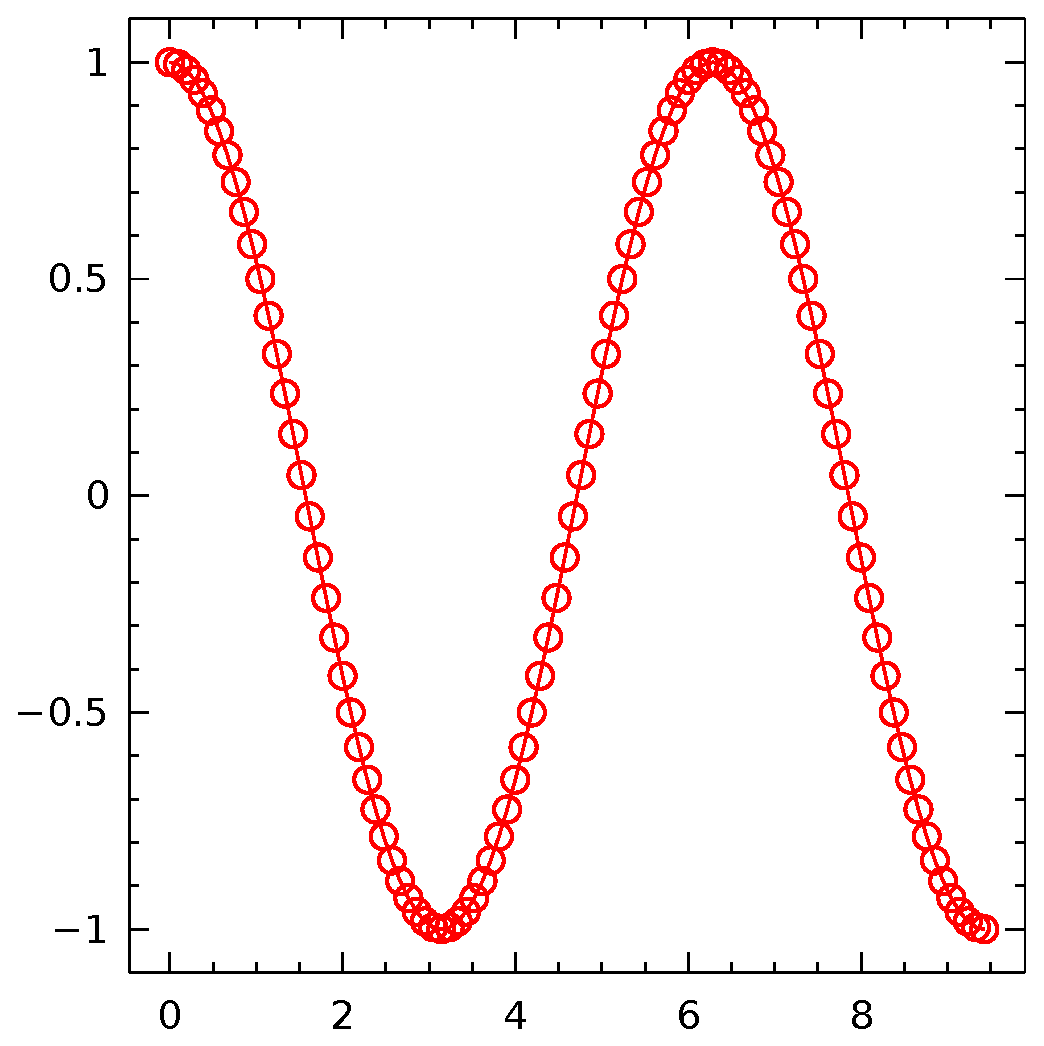
\includegraphics{winston-coseno}
\caption{Ejemplo de gráfico en Winston}
\label{fig:winston-coseno}
\end{figure}

El primer argumento (vector de puntos en el eje $X$) es opcional: si solo se pasa un vector de datos, estos se dispondrán como si el eje $X$ fuese \code{[1:length(y)]}. El tercer argumento (también opcional) es una cadena de texto que indica los atributos gráficos de la serie dibujada (por defecto una linea continua negra). En este caso, una línea continua (\code{'-'}), con puntos marcados como círculos (\code{'o'}), todo ello de color rojo (\code{'r'}). Estos atributos pueden consistir en tipos de linea, marcas de puntos, o colores (figura \ref{fig:winston-modificadores}), y se pueden combinar en cualquier orden, con una excepción: \code{"-."} representa ``linea discontinua alternada con puntos'', mientras que \code{".-"} equivale a ``marcadores en forma de puntos'' + ``linea continua''.

\begin{figure}
\centering
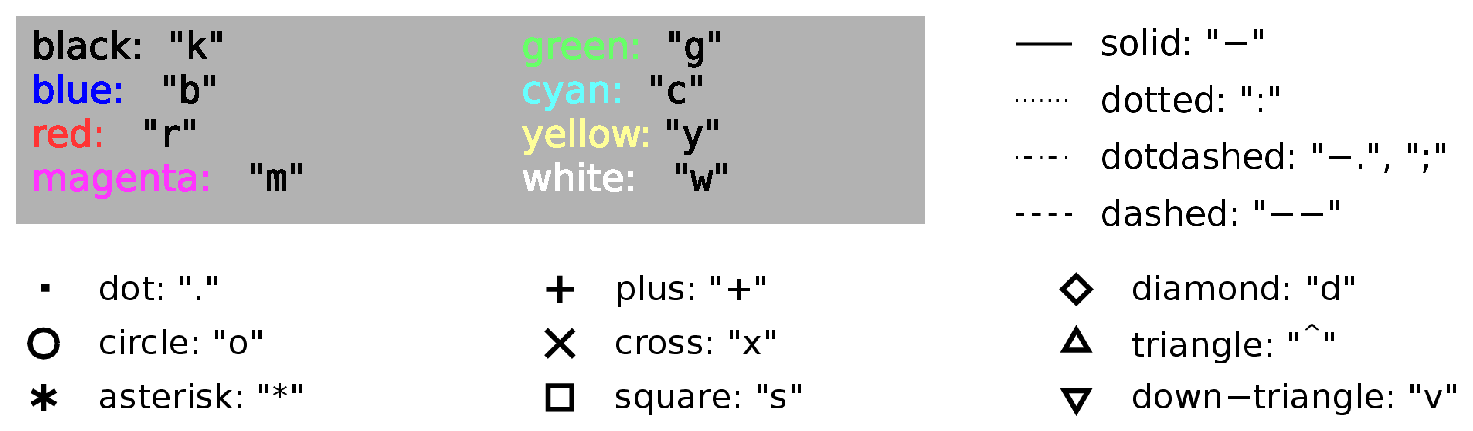
\includegraphics[width=0.8\textwidth]{winston-modificadores}
\caption{Especificaciones de colores, líneas y marcadores}
\label{fig:winston-specs}
\end{figure}


La función \code{plot}, además de representar el gráfico especificado en pantalla, crea en memoria un objeto de la clase \code{FramedPlot} con los contenidos del gráfico, que es el valor devuelto por la función. Es decir, que si hubiéramos escrito, por ejemplo:

\begin{jlconcode}
julia> p = plot(x, y, "-or")
\end{jlconcode}

la variable \code{p} contendría los contenidos del gráfico en cuestión. De este modo, si se cierra la ventana del gráfico o se cambia su contenido, este se puede volver a mostrar invocando a esta variable.

\section{Series de datos superpuestas}

Asignar un gráfico a una variable también sirve para añadirle nuevas series de datos u otros componentes. Si a la función \code{plot} le añadimos un primer argumento con el contenido de un gráfico anterior:

\begin{jlconcode}
julia> # Dibujar sobre el gráfico "p"
julia> plot(p, x, sin(x))
\end{jlconcode}

veremos una nueva linea dibujada sobre la anterior (figura \ref{fig:winston-superposicion}). Si no se hubiera especificado ese primer argumento, simplemente se habría creado un nuevo gráfico que sustituiría al anterior, en lugar de superponerse.

\begin{figure}
\centering
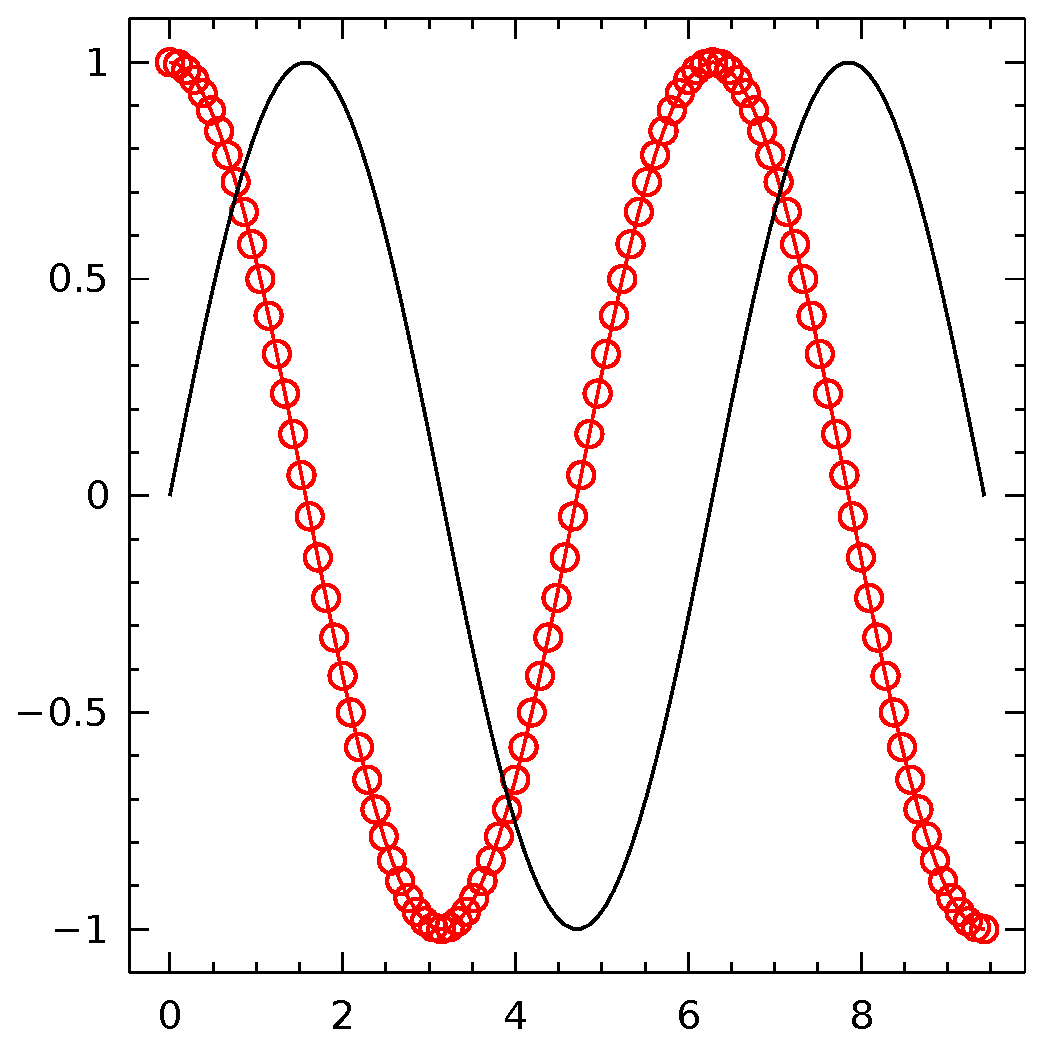
\includegraphics{winston-coseno-seno}
\caption{Superposición de gráficos}
\label{fig:winston-superposicion}
\end{figure}

Esta forma de añadir componentes es especialmente útil si se trabaja con varios gráficos a al vez. Si solo se trabaja con uno, basta con utilizar la función \code{oplot} (forma abreviada de \emph{overplot}), que funciona igual que \code{plot} pero siempre añade la serie de datos especificada al último gráfico que se haya creado.

Otra opción es emplear la función \code{hold}, que altera el comportamiento de \code{plot} en este aspecto:

\begin{jlconcode}
julia> hold(false) # comportamiento por defecto de "plot"
julia> hold(true)  # cambia "plot" para hacer lo mismo que "oplot"
julia> hold()      # alterna ambos comportamientos de "plot"
\end{jlconcode}

Alternativamente, se puede llamar a \code{plot} especificando múltiples series de datos, para que las represente superpuestas en un solo paso.

\begin{jlconcode}
julia> # Esta instrucción también genera el gráfico con dos líneas
julia> plot(x, y, "-or", x, sin(x), "k")
\end{jlconcode}

Como se ve en el ejemplo, los grupos de argumentos (datos en el eje $X$, datos en el eje $Y$, y atributos visuales) se añaden secuencialmente. Los argumentos opcionales (eje $X$ y atributos) se pueden omitir si la secuencia resultante no es ambigua.

Y también hay otra alternativa más sencilla en el caso de que las series de datos tengan la misma longitud: juntar los valores del eje $Y$ en una sola matriz, con cada serie en una columna. La función \code{plot} asigna a cada columna un color distinto por defecto, repitiéndose esta secuencia cada 8 columnas: (1) negro, (2) rojo, (3) verde, (4) azul, (5) naranja, (6) morado/índigo, (7) marrón, (8) violeta/púrpura.

\begin{jlconcode}
julia> # seno en una línea negra, coseno en una línea roja
julia> plot(x, [sin(x) cos(x)])
\end{jlconcode}

\section{Trabajar con múltiples figuras}

Para trabajar con más de un gráfico en pantalla, se deben abrir distintas figuras o ventanas gráficas.%
\footnote{%
Esto es así al menos cuando se trabaja con la interfaz básica de Julia. Los distintos IDEs pueden cambiar la forma de visualizar los gráficos.%
}
Conviene tener clara la diferencia entre los conceptos de ``figura'' y ``gráfico'' (en términos técnicos, \emph{Figure} y \emph{FramedPlot}, respectivamente). El segundo es siempre un contenido de la primera, como se muestra en la figura XXX.

Para crear una nueva figura se utiliza la función \code{figure} sin ningún argumento. Esta función devuelve un número entero que identifica a la figura mientras esta se encuentre abierta. Además hará que esa figura sea la ``activa'', es decir que que desde ese momento todas las operaciones gráficas se hagan sobre ella y sus contenidos.

\begin{jlconcode}
julia> # Crear una nueva figura y asignar su identificador a f
julia> f = figure()
\end{jlconcode}

Si posteriormente se crean otras figuras, se puede volver a activar una anterior, empleando este identificador como argumento de \code{figure}:

\begin{jlconcode}
julia> # f vuelve a ser la figura activa
julia> figure(f)
\end{jlconcode}

La operación complementaria de eliminar una figura creada se lleva a cabo con la función \code{closefig} (aparte de la posibilidad hacer ``click'' sobre el botón para cerrar la figura, cuando se trabaja en modo interactivo):

\begin{jlconcode}
julia> # Cerrar la figura f
julia> closefig(f)
\end{jlconcode}

Es importante mencionar que las figuras recién creadas están ``vacías''; no contienen ningún gráfico, ni siquiera en blanco, hasta que se llama a la función \code{plot} o una equivalente. Esto significa que la función \code{oplot} no actuará sobre ellas. Y tampoco se puede utilizar el identificador de la figura como primer argumento de \code{plot}, ya que se trata de un objeto de distinto tipo. Si se quiere, para crear un gráfico en blanco se puede emplear a la función ``constructora'' \code{FramedPlot}.

Por otro lado, si no hay ninguna figura abierta, las funciones como \code{plot}, \code{FramedPlot}, etc. la crean automáticamente, aunque no dan información sobre ella. Si hace falta, el identificador de la figura activa se puede recuperar con la función \code{gcf} ---sin argumentos---, cuyo nombre representa el acrónimo de \emph{get current figure}.

\begin{jlconcode}
julia> # f identifica a la figura que contiene el gráfico p
julia> p = plot(x, y)
julia> f = gcf()
\end{jlconcode}


\section{Tablas de gráficos, decoraciones y otras complejidades}

Para mostrar de forma práctica otros aspectos de la composición de gráficos, a continuación se plantea un ejemplo algo más complejo, que incluye un par de rutinas habituales: la definición de ``decoraciones'' como títulos, leyendas o etiquetas de los ejes, ajustar el rango de los ejes, y organizar una tabla de gráficos en la misma figura. Este ejemplo también sirve para ver el uso de algunas operaciones rutinarias en cálculos numéricos.

El ejemplo consiste en una composición de dos gráficos (figura \ref{fig:winston-ejemplo-completo}): el gráfico superior muestra una señal de frecuencia modulada y amplitud amortiguada (línea negra), a la que se le ha añadido un error aleatorio (puntos grises), y se ha ajustado con una media ponderada móvil (línea roja). El aspecto más ``ruidoso'' de la señal ajustada en el tramo final se representa en forma de razón entre señal y ruido (\emph{signal-to-noise ratio}, SNR) en el panel inferior. El código para generar este gráfico es el siguiente:

\begin{figure}
\centering
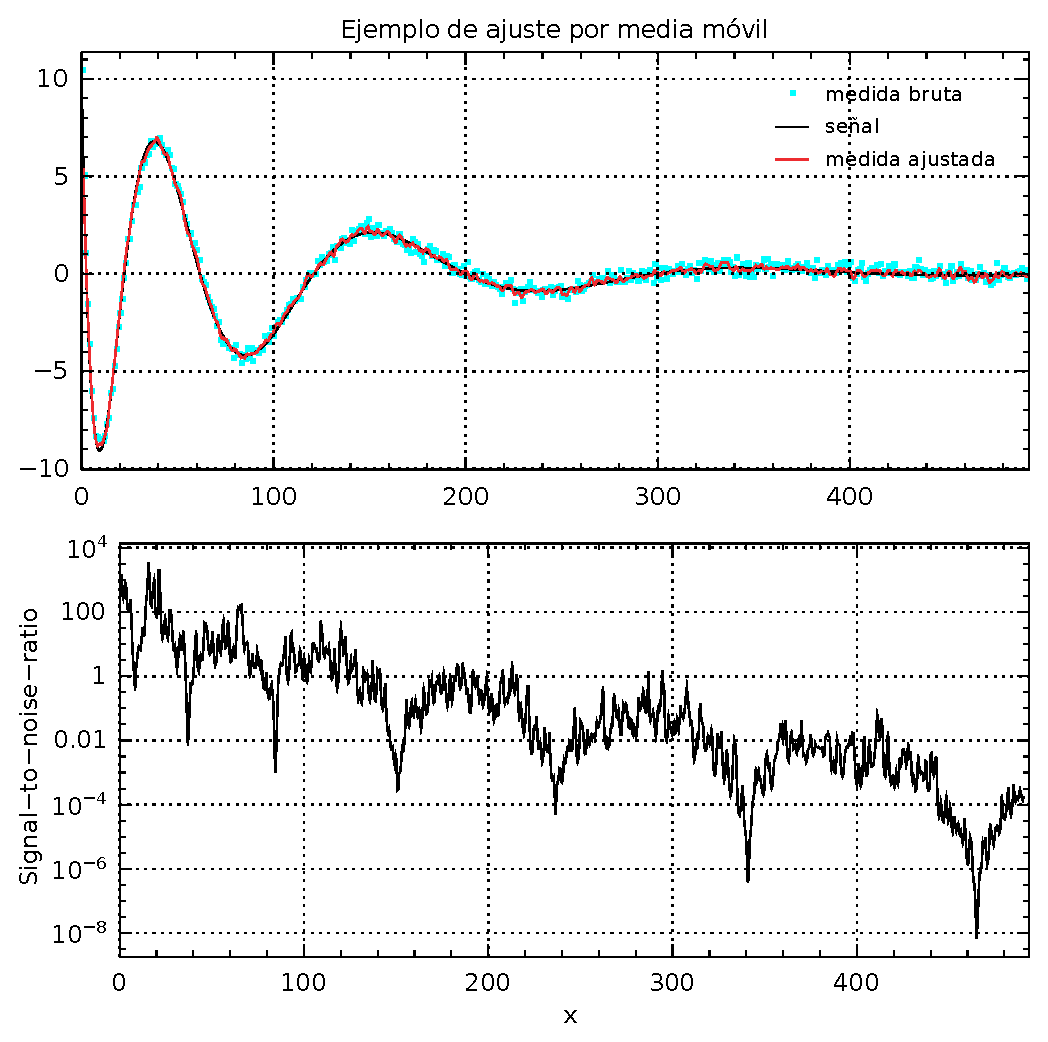
\includegraphics{winston-ejemplo-completo}
\caption{Ejemplo de composición de gráficos}
\label{fig:winston-ejemplo-completo}
\end{figure}

\begin{juliacode}
# x es la variable independiente
x = linspace(0, 50pi^2, 1000)
# f = señal ideal, y = señal observada
f = 10cos(sqrt(x)) .* exp(-x/100)
y = f+0.25randn(1000)
# yfit = señal ajustada con una media ponderada móvil
yfit = fill(NaN, 1000)
b = [1, 2, 3, 2, 1]/9
for t = 3:998
  yfit[t] = sum(y[t-2:t+2] .* b)
end
# Signal-to-noise ratio
# (ver comentario)
signal_pow = fill(NaN, 1000)
noise_pow = fill(NaN, 1000)
noise = yfit - f
for t = 3:998
  signal_pow[t] = sum((f[t-2:t+2] - mean(f[t-2:t+2])).^2)
  noise_pow[t] = sum((noise[t-2:t+2] - mean(noise[t-2:t+2])).^2)
end
snr = (signal_pow./noise_pow)[5:end]
# Aquí empiezan los gráficos
plottable = Table(2, 1)
plottable[1,1] = plot(x[1:2:end], y[1:2:end], ".c", x, [f yfit])
xlim(0,50pi^2)
title("Ejemplo de ajuste por media móvil")
grid(true)
legend(["medida bruta", "señal", "medida ajustada"], 0.75, 0.9)
plottable[2,1] = semilogy(x[3:end-2], snr)
xlim(0,50pi^2)
xlabel("x")
ylabel("Signal-to-noise-ratio")
grid(true)
plottable
savefig(plottable, "figura.png")
\end{juliacode}

Las primeras líneas de este ejemplo son las operaciones realizadas para obtener los datos del panel superior. Se usa la función \code{linspace} para crear un vector de 1000 puntos equiespaciados entre $0$ y $50\pi$, unas sencillas funciones matemáticas para la señal ideal, y la función \code{randn} para añadirle el ruido aleatorio (procedente de una distribución gaussiana).

Este ruido se intenta cancelar con una media ponderada móvil, de ventana triangular de 5 puntos representada por el vector de coeficientes \code{b}. Este último cálculo se realiza con el bucle \code{for}, que es autoexplicativo --- los detalles de esta técnica se presentan en  el siguiente capítulo.%
\footnote{%
Sería mucho más eficiente hacer esta operación con la
función \code{filt}, pero se opta por esta solución más trivial para no
complicar el ejemplo con cuestiones relativas al tratamiento de señales digitales.%
}
Los dos primeros y últimos puntos de la señal ajustada no se calculan, y se dejan como \emph{not-a-numbers} (\code{NaN}), para evitar ``efectos de borde''. Luego se calcula la medida en que varían la señal original y la filtrada para obtener la SNR. Estas variaciones se calculan como una ``suma de cuadrados móvil'' con un ancho de 5 puntos. Esto se hace con un bucle semejante al usado para la media ponderada móvil.

A esto le siguen las operaciones gráficas. Para construir una tabla de gráficos se emplea la función \code{Table} con dos argumentos: el número de filas y columnas de la tabla, respectivamente. El valor devuelto es un objeto del tipo \code{Winston.PlotContainer}. La gráfica creada con la función \code{plot} se asigna al panel que corresponde de esta tabla, del mismo modo que si trabajásemos con \emph{arrays} de datos numéricos.

En este ejemplo, la primera llamada a \code{plot} se utiliza para representar tres series de datos al mismo tiempo. La primera secuencia es la de los puntos observados (\code{".c"} son puntos en color cian), representados de dos en dos para que el gráfico sea menos denso. La segunda secuencia son las dos líneas con la señal original y la ajustada, puestas como un solo conjunto de datos en forma de matriz.

El panel inferior representa la razón entre señal y ruido (\code{snr}), pero en lugar de \code{plot} se utiliza la función \code{semilogy}, porque queremos que el eje Y se represente en escala logarítmica para visualizar mejor cómo varía esta medida. Para poner en escala logarítmica el eje X o ambos, se emplean las funcioines \code{semilogx} y \code{loglog}, respectivamente.

También se muestra el uso de algunas funciones habituales para ajustar los límites del gráfico y ``decorar'' el contexto. (véase que estas funciones se han llamado tras crear los objetos gráficos del panel que se quiere modificar):

\begin{itemize}
  \item \code{xlim} define los límites inferior y superior del eje $X$ (el eje $Y$ se ajusta con \code{ylim})
  \item Las funciones \code{title}, \code{xlabel}, \code{ylabel} sirven para añadir texto al título y los dos ejes, respectivamente
  \item \code{grid} se emplea para añadir o eliminar la cuadrícula en el area gráfica
  \item \code{legend} añade una leyenda con los textos especificados para las distintas series de datos representadas; el primer argumento es un vector de cadenas de texto, ordenadas según se han creado los elementos gráficos que se etiquetan en la leyenda; los dos siguientes argumentos son las coordenadas de la ``caja'' que contiene la leyenda, relativas al área de la figura ($(0,0)$ representa la esquina inferior izquierda, y $(1,1)$ la superior derecha).
\end{itemize}

Hacia el final se llama a la tabla de gráficos por su nombre, para mostrar el resultado una vez terminado el proceso. El motivo es que si las líneas del código se ejecutan una a una en modo interactivo, se verá que al llamar a la función \code{Table} aparece una figura en blanco; luego, cuando se crea cada uno de los gráficos, estos sustituyen a la figura vacía ocupando toda la ventana gráfica. La tabla con los dos gráficos combinados solo aparece al volver a llamar a la tabla de gráficos al final. Este comportamiento recalca la importancia de asignar el objeto devuelto por \code{Table} a una variable, ya que para visualizar la tabla de gráficos hay que llamarla explícitamente después de crearla. Ni siquiera ocultando los dos gráficos individuales (por ejemplo añadiendo un punto y coma tras las líneas segunda y tercera) se hubiera actualizado la vista de la tabla, hasta llamar la última línea.

Finalmente, para salvar el resultado a un archivo gráfico, basta con darle el nombre del archivo a la función \code{savefig}. Los tipos de archivo soportados por la función son EPS, PDF, SVG y PNG. El identificador del gráfico es opcional ---por defecto se imprime el gráfico de la figura activa---, y en el caso de guardarse un archivo de tipo PDF, se puede asignar un vector de gráficos (objetos de tipo \code{PlotContainer}), cada uno de los cuales se imprimirá en una página distinta.


\section{Edición de gráficos}

De vez en cuando se desea cambiar algún atributo de las gráficas creadas, lo cual puede conseguirse habitualmente con las funciones \code{setattr} y \code{style}.

Su uso se muestra algunos ejemplos que pueden ser más o menos habituales, siguiendo con el caso mostrado en la sección anterior. La lista completa de atributos asignados a cada tipo de objeto se puede encontrar en la referencia del paquete Winston (\url{https://github.com/nolta/Winston.jl/wiki/Reference}), así como otros ejemplos en \url{http://winston.readthedocs.org/}. También se pueden visualizar la estructura de un gráfico, incluyendo sus atributos, con la función \code{dump}:

\begin{jlconcode}
julia> dump(plottable[1,1])
Winston.FramedPlot 
  attr: Dict{Any,Any} len 6
    title_offset: Float64 1.0
    page_margin: Float64 0.1
    gutter: Float64 0.1
    aspect_ratio: Void nothing
    title: UTF8String "Ejemplo de ajuste por media móvil"
    title_style: Dict{Symbol,Any} len 1
      fontsize: Float64 3.0
  content1: Winston.PlotComposite 
    attr: Dict{Any,Any} len 1
      style: Dict{Symbol,Any} len 0
    components: Array(Any,(4,))
      1: Winston.Points 
        attr: Dict{Any,Any} len 2
          style: Dict{Symbol,Any} len 3
          label: UTF8String "medida bruta"
        x: LinSpace{Float64} 
          start: Float64 0.0
          stop: Float64 492.9862458602192
          len: Float64 500.0
          divisor: Float64 499.0

[Output truncado]
\end{jlconcode}

En el fragmento mostrado se ven los 6 atributos del panel superior, del que el más obvio es el título (\code{title}). Por lo tanto, si se quisiera editar el título en cualquier momento (por ejemplo para ponerlo en mayúsculas):

\begin{jlconcode}
julia> # Con getattr se obtiene el valor actual del atributo
julia> titulo = getattr(plottable[1,1], "title")
"Ejemplo de ajuste  media móvil"
julia> # Lo convertimos en mayúscula, y lo reasignamos con setattr
julia> # usando el argumento con el nombre correspondiente
julia> setattr(plottable[1,1], title=uppercase(titulo))
julia> # Volvemos a llamar al gráfico para que se vea el resultado
julia> plottable
\end{jlconcode}

También se pueden ver las series de datos representadas por los objetos dentro del vector \code{components} en el campo \code{content1} (en el fragmento mostrado se ven las primeras líneas referidas a la serie de puntos).%
\footnote{%
Todo gráfico tiene sus contenidos distribuidos en \code{content1} y
\code{content2}. En los más habituales todo se encuentra dentro de
\code{content1}.%
}
El conjunto de componentes se puede extraer con la función \code{getcomponents}, para facilitar su edición.

\begin{jlconcode}
julia> comp = getcomponents(plottable[1,1])
4-element Array{Any,1}:
 Winston.Points(...)
 Winston.Curve(...) 
 Winston.Curve(...) 
 Winston.Legend(...)
\end{jlconcode}

Las propiedades visuales de las series de datos, como el tipo y color de las líneas y los puntos, están en un atributo especial llamado \code{style} (estilo):

\begin{jlconcode}
julia> # Atributos del primer componente (serie de puntos)
julia> # El campo "attr" del objeto "xxx" se extrae como "xxx.attr"
julia> dump(comp[1].attr)
Dict{Any,Any} len 2
  style: Dict{Symbol,Any} len 3
    symbolkind: ASCIIString "dot"
    color: ColorTypes.RGB{FixedPointNumbers.UFixed{UInt8,8}} 
      r: FixedPointNumbers.UFixed{UInt8,8} 
        i: UInt8 0
      g: FixedPointNumbers.UFixed{UInt8,8} 
        i: UInt8 255
      b: FixedPointNumbers.UFixed{UInt8,8} 
        i: UInt8 255
    symbolsize: Float64 1.0
  label: UTF8String "medida bruta"

julia> # Lo mismo para las dos líneas
julia> dump(comp[2].attr)
Dict{Any,Any} len 3
  style: Dict{Symbol,Any} len 2
    linecolor: UInt32 0
    linewidth: Float64 2.0
  label: UTF8String "señal"
  kw_defaults: Dict{Symbol,Any} len 1
    linewidth: Float64 2.0

julia> dump(comp[3].attr)
Dict{Any,Any} len 3
  style: Dict{Symbol,Any} len 2
    linecolor: UInt32 15543344
    linewidth: Float64 2.0
  label: UTF8String "medida ajustada"
  kw_defaults: Dict{Symbol,Any} len 1
    linewidth: Float64 2.0
\end{jlconcode}

Supongamos que para resaltar los aspectos de interés, queremos convertir el color de los puntos a gris, presentar la señal ideal como una línea roja discontinua gruesa, y la medida ajustada como una línea azul más delgada (figura \ref{fig:winston-ejemplo-modificado}). Para ello utilizaremos las siguientes instrucciones:

\begin{jlconcode}
julia> style(comp[1], color="grey")
julia> style(comp[2], linekind="dashed", linecolor="red", linewidth=3)
julia> style(comp[3], linewidth=1.5, linecolor="blue")
julia> plottable
\end{jlconcode}

\begin{figure}
\centering
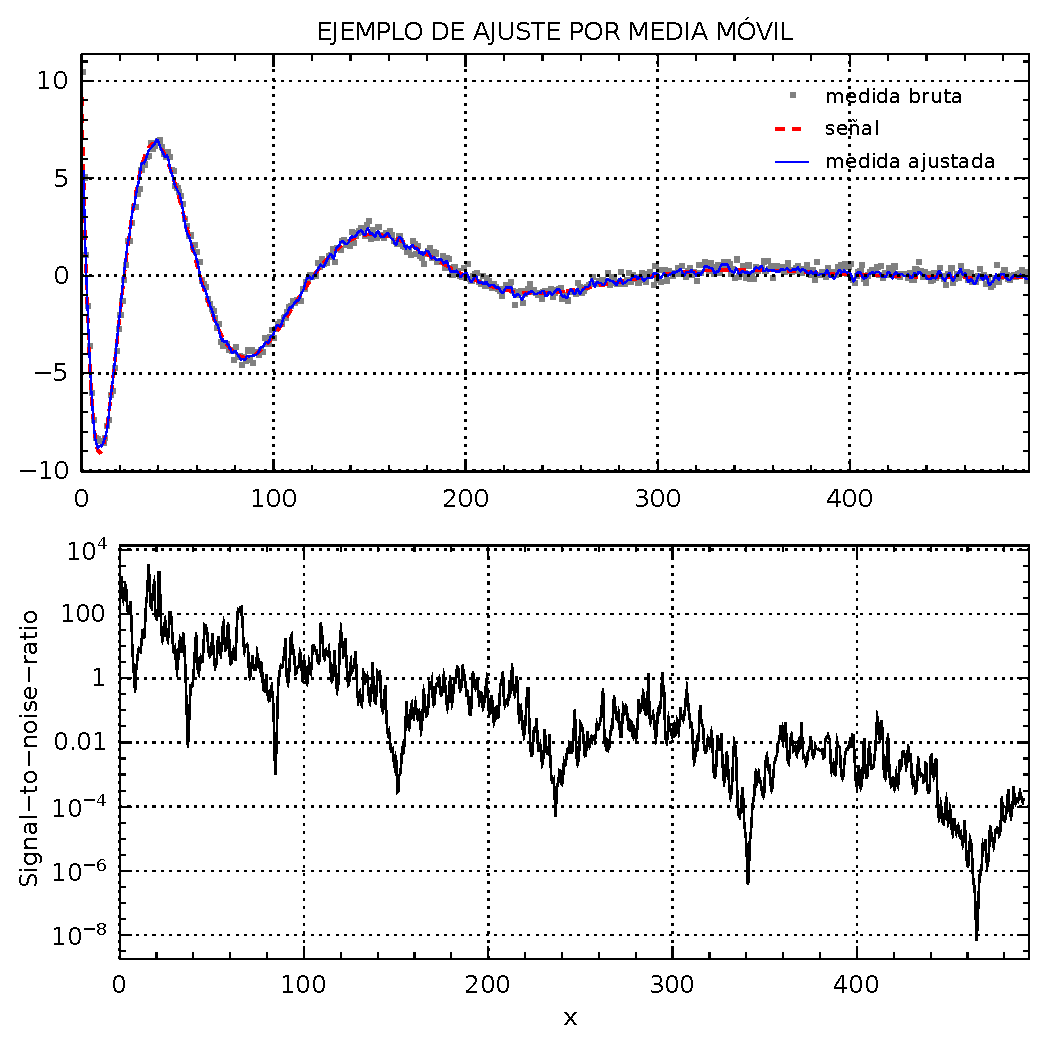
\includegraphics{winston-ejemplo-modificado}
\caption{Superposición de gráficos}
\label{fig:winston-ejemplo-modificado}
\end{figure}

\section{Otros gráficos}

La función \code{plot} es la más habitual para representar series de datos, pero también hay más funciones para otro tipo de representaciones, entre otras:

\begin{itemize}
  \item \code{stem}: gráficos de ``tallos''. Representan series de datos, al igual que \code{plot}, pero se añaden líneas verticales que conectan cada punto con el eje $Y=0$.
  \item \code{scatter}: gráficos de dispersión. Se diferencia de \code{plot} en que es necesario especificar los valores en el eje $X$, por defecto se representan puntos, no líneas, y también se pueden introducir variables que especifican el tipo y el color de cada punto individual.
  \item \code{errorbar}: barras de error. A los valores del eje $X$ e $Y$ se les añade el argumento \code{xerr} o \code{yerr}, según si se quieren representar barras horizontales o verticales, respectivamente. Este argumento ha de escribirse con el nombre explícito, para evitar ambigüedades. Si la serie de datos contiene $n$ puntos, este argumento ha de ser un vector numérico de longitud $n$ (para barras simétricas) o $2n$ (para especificar distintas amplitudes en ambas direcciones a partir de los puntos especificados). En este último caso, los valores de $1$ a $n$ del argumento adicional representa cuánto se extiende la barra hacia la izquierda (para \code{xerr}) o hacia abajo (para \code{yerr}), y del $n+1$ hasta el $2n$ cuánto se extiende hacia la derecha o hacia arriba, respectivamente.
  %\item \code{bar}, \code{barh}: diagramas de barras verticales y horizontales, respectivamente. El primer argumento especifica las etiquetas que se presentan en los valores del eje $X$ ($Y$ para las barras horizontales). El segundo representa las alturas de cada barra; si es una matriz $N\times{}M$, se presentan $N$ grupos de $M$ barras coloreadas.
  \item \code{plothist}: histogramas. Se le pasa un vector de datos, e internamente usa la función \code{hist} para definir los intervalos del eje $X$ y calcular las frecuencias del vector en esos intervalos. Como en esa función, se puede definir el número (aproximado) de barras o los límites exactos de las mismas añadiendo dichos valores como argumentos adicionales.
  \item\code{hist2d}: histograma bidimensional. En este caso se le pasa una matriz de dos columnas, y los ejes $X$, $Y$ de la imagen se asocian a los intervalos de la primera y la segunda columna, respectivamente. Las frecuencias para cada combinación de intervalos se representan en una escala de color.
  \item\code{imagesc}: mapas de color a partir de una matriz de datos. Los argumentos requeridos son, en orden: el intervalo en el eje $X$, el intervalo en el eje $Y$, la matriz de datos a representar ($X$ en filas, $Y$ en columnnas), y el intervalo de valores de la matriz al que se ajusta la escala de colores. El único argumento requerido es la matriz de datos, y los omitidos se calculan automáticamente.
\end{itemize}

Las funciones \code{hist2d} o \code{imagesc} utilizan ``mapa de color'' para representar los datos. Por defecto el mapa empleado es el llamado \emph{jet} o ``arcoiris''. Este mapa de colores se puede cambiar por una escala de degradados de distintos colores, a través de la función \code{colormap} --- que se ha de llamar \emph{antes} de crear el gráfico:

\begin{juliacode}
colormap("blues")   # Escala de azules
colormap("greens")  # Escala de verdes
colormap("grays")   # Escala de grises
colormap("oranges") # Escala de naranjas
colormap("purples") # Escala de púrpuras
colormap("reds")    # Escala de rojos
\end{juliacode}

\chapter{Condiciones y bucles}

\section{\code{if}, \code{while}, \code{for}...}

En algunos ejemplos de los capítulos anteriores ya se han presentado modelos de sentencias condicionales y bucles. Esos ejemplos se han dado sin apenas explicaciones, en parte por ser prácticamente autoexplicativos, pero también porque ya no solo el concepto, sino también su sintaxis son prácticamente un estándar fácilmente reconocible por todo lector con una mínima experiencia previa en programación.

Sin embargo, es imperativo para cualquier guía introductoria de programación dar en algún punto cuenta de los bloques condicioneales y los distintos tipos de bucles, ya que estamos hablando de las estructuras que controlan el ``flujo'' que sigue la ejecución del código, y junto a la asiganción de valores a variables, vienen a ser el fundamento de cualquier lenguaje de programación. Por otro lado, este tema también nos sirve para introducir otras estructuras y detalles específicos de Julia.

Así pues, si bien sea por no dejarlas de mencionar, comenzamos presentando la sintaxis básica de estas estructuras:

\textbf{Bloques condicionales (\code{if}):}

\begin{juliacode}
if condición
  # Código que se ejecuta si se cumple "condición"
end
\end{juliacode}

\textbf{Bucles tipo \code{while}:}

\begin{juliacode}
while condición
  # Código que se ejecuta de forma repetida
  # mientras se siga cumpliendo "condición"
end
\end{juliacode}

\textbf{Bucles tipo \code{for}:}

\begin{juliacode}
for i = serie
  # Código que se ejecuta de forma repetida
  # empleando la variable "i" con el valor de cada uno
  # de los elementos iterables de la variable "serie".
end

for i in serie
  # Exactamente lo mismo que lo anterior
  # utilizando la palabra clave "in" en lugar de "=".
end
\end{juliacode}

Cabe mencionar que estas estructuras requieren usar las variables aquí ejemplificadas como "condición" y "serie", que han de ser de un tipo especial en cada caso: las condiciones han de ser variables lógicas, y las series variables iterables. Se entrará más en detalle sobre estos tipos de variables en las próximas secciones.

Antes, conviene adelantar algunas ``extensiones'' a la sintaxis básica, que sin ser imprescindibles, facilitan mucho la creación de estas estructuras de control de flujo.

En primer lugar están las condiciones alternativas (\code{else}, \code{elseif}). Tras un bloque condicionado por \code{if}, se pueden intercalar otros bloques de código a ejecutar si se cumplen otras condiciones:

\begin{juliacode}
if condición1
  # Ejecutar este bloque si se cumple "condicion1"
elseif condición2
  # Ejecutar este bloque si no se cumple la condición anterior,
  # pero sí se cumple "condicion2"
  # Se pueden poner tantas condiciones alternativas como se quiera...
  # ...
else
  # Bloque que se ejecuta si no se cumple *ninguna*
  # de las condiciones enunciadas
end
\end{juliacode}

La función \code{ifelse} también sirve como alternativa a la estructura \code{if}/\code{else} para algunos casos sencillos. Por ejemplo, esta forma de comprobar si un número se puede considerar entero (aunque esté codificado como decimal):

\begin{juliacode}
# Comprobación con estructura if/else
if mod(numero,1) == 0
  print("Es un número entero")
else
  print("Es un número decimal")
end

# Comprobación con la función ifelse
print(ifelse(mod(numero,1)==0, "Es un número entero", "Es un número decimal"))
\end{juliacode}

Por otro lado, están los comandos \code{break} y \code{continue} para alterar el flujo habitual de los bucles. Estos comandos suelen ir en un \code{if} dentro de un bucle \code{while} o \code{for}. \code{break} interrumpe el bucle en el punto en que se encuentre, y devuelve el control al segmento de código desde el que se llamó el bucle, como si este hubiera terminado. \code{continue} hace algo semejante, pero solo interrumpe una iteración, y salta al comienzo de la siguiente. Veamos un ejemplo práctico, en un código para calcular los números primos del 1 al 100 mediante una implementación literal de la ``criba de Eratóstenes'':%
\footnote{%
\url{https://es.wikipedia.org/wiki/Criba_de_Eratóstenes}%
}

\begin{quote}
Se forma una tabla con todos los números naturales comprendidos entre $2$ y $n$, y se van tachando los números que no son primos de la siguiente manera: Comenzando por el 2, se tachan todos sus múltiplos; comenzando de nuevo, cuando se encuentra un número entero que no ha sido tachado, ese número es declarado primo, y se procede a tachar todos sus múltiplos, así sucesivamente. El proceso termina cuando el cuadrado del mayor número confirmado como primo es mayor que $n$.
\end{quote}

\begin{juliacode}
n = 100
# Utilizamos como "criba" un vector lógico,
# con todos los valores inicialmente definidos como "false"
eliminados = falses(n)
# Comenzando por 2...
for m = 2:n
  # Si el número (m) ha sido eliminado, pasar al siguiente
  if eliminados[m]
    continue
  end
  # Eliminar los múltiplos 2m, 3m ... menores que n
  k = 2
  while (mxk = m*k) <= n
    eliminados[mxk] = true
    k += 1
  end
  # Terminar si el cuadrado de m es mayor que n 
  if m^2 > n
    break
  end
end
# Extraer las posiciones no eliminadas de la criba
# (usando el operador "~" para convertir true en false, y viceversa
primos = find(~eliminados)
\end{juliacode}

\section{Expresiones lógicas}

La condición asociada a los bloques \code{if} o \code{elseif}, así como a los bucles \code{while}, ha de expresarse en una variable lógica, de tipo \code{Bool}, que no es otra cosa que un número binario, cuyos valores posibles son \code{true} y \code{false}. Estos valores lógicos se pueden obtener de múltiples maneras. Posiblemente la más habitual es a partir de comparaciones:
\code{==} (igual), \code{!=} (distinto),
\code{>} (mayor), \code{>=} (mayor o igual),
\code{<} (menor), \code{<=} (menor o igual), etc.

Sin embargo, también hay muchas otras funciones que dan como resultado variables lógicas, como resultado de comprobar ciertas condiciones numéricas o de otro tipo. Algunas que pueden usarse habitualmente son:

\begin{description}
  \item[\code{isdefined(x)}] \hfill \\
  Comprobar si existe la variable identificada por el símbolo \code{x} en el espacio de trabajo. Si una variable tiene por ejemplo el nombre \code{v}, el ``símbolo'' que la identifica es \code{:v} (con dos puntos); es decir, que la forma de llamar a la función sería \code{isdefined(:v)}.
  \item[\code{isdefined(x,index)}] \hfill \\
  Si \code{x} es un \emph{array} u otro tipo de variable compuesta por varios componentes, se interroga si esa variable contiene el componente representado por el índice \code{index}; p.ej. \code{isdefined(v, 5)} para comprobar si existe un quinto elemento en \code{v}.
  \item[\code{isnan(x)}] \hfill \\
  Comprobar si \code{x} es un \code{NaN} (\emph{not-a-number)}.
  \item[\code{isfinite(x)}, \code{isinf(x)}] \hfill \\
  Comprobar si \code{x} es un número finito o infinito, respectivamente. (Un \code{NaN} devuelve \code{false} para ambas funciones.)
  \item[\code{isinteger(x)}] \hfill \\
  Comprobar si \code{x} es un número entero, u otro tipo de variable (p.ej. un vector) que solo contiene números enteros.
  \item[\code{isreal(x)}] \hfill \\
  Comprobar si \code{x} es un número real, u otro tipo de variable (p.ej. un vector) que solo contiene números reales.
  \item[\code{iseven(x)}, \code{isodd(x)}] \hfill \\
  Comprobar si \code{x} (que ha de ser un número entero) es par o impar, respectivamente.
  \item[\code{isempty(x)}] \hfill \\
  Aplicable a vectores u otro tipo de ``colecciones'' (véase la siguiente sección). Comprueba si \code{x} está vacío (no tiene ningún elemento).
  \item[\code{isa(x,type)}] \hfill \\
  Comprobar si la variable \code{x} es del tipo \code{type}, p.ej. \code{isa(x, Number)}, \code{isa(x, Bool)},\ldots (ver la sección XXXX sobre tipos).
  \item[\code{iseltype(x,type)}] \hfill \\
  Equivalente a \code{isa}, pero también válido para \emph{arrays} u otro tipo de colecciones; en el segundo caso comprueba el tipo de todos sus elementos.
  \item[\code{in(el,x)}] \hfill \\
  Comprobar si el elemento con el valor \code{el} está presente en la colección \code{x}.
  \item[\code{any(x)}] \hfill \\
  Si \code{x} es un \emph{array} con elementos de tipo \code{Bool}, comprobar si al menos uno de los elementos es \code{true}.
  \item[\code{all(x)}] \hfill \\
  Si \code{x} es un \emph{array} con elementos de tipo \code{Bool}, comprobar si todos los elementos son \code{true}.
\end{description}

Volviendo a los operadores lógicos de comparación, una característica interesante de Julia es que permite concatenarlos como se hace a menudo al escribir relaciones matemáticas. Por ejemplo, para verificar si un valor de probabilidad \code{p} está efectivamente acotado entre \code{0} y \code{1}:

\begin{jlconcode}
julia> p = 0.5;
julia> 0 <= p <= 1
true
\end{jlconcode}

Estas comparaciones se pueden hacer también sobre los distintos elementos de un \emph{array}, pero para hacer la comparación elemento a elemento hay que utilizar los operadores ``con punto'' (cfr. la sección XXXXX). Los resultados de estas comparaciones son vectores lógicos, que no se pueden usar como condición en un \code{if} o \code{while} (estos solo admiten valores de tipo \code{Bool} unitarios), pero se usan a menudo para seleccionar elementos de otro vector y operar sobre ellos. Por ejemplo, veamos la siguiente alternativa al bucle \code{while} del ejemplo anterior, que también nos sirve para introducir otros detalles sobre las expresiones lógicas:

\begin{juliacode}
multiplos_m = (mod([1:n], m) .== 0)
igual_a_m = ([1:n] ~= m)
eliminados[multiplos_m & igual_a_m] = true
\end{juliacode}

La primera línea contiene una de estas comparaciones lógicas con \emph{arrays}. Concretamente calcula un vector de \code{Bool}, que son \code{true} para los múltiplos de \code{m} (dan resto igual a cero al dividirlas por \code{m}). La segunda línea utiliza el operador \code{~=}, que es el equivalente a \code{!=} (``distinto de'') para \emph{arrays}; el resultado es otro vector de \code{Bool} igual a \code{true} en todas las posiciones salvo \code{m}. En la tercera línea se seleccionan los elementos de \code{eliminados} que cumplen ambas condiciones: múltiplos de \code{m} con excepción de \code{m}, y se les asigna el valor \code{true}.%
\footnote{%
El paréntesis alrededor de las expresiones lógicas es opcional, ya que las operaciones lógicas tienen precedencia sobre otras, pero en estos ejemplos se usan los paréntesis de forma generalizada para facilitar la lectura y la interpretación de las expresiones.%
}

Como en este ejemplo, las expresiones lógicas a menudo se componen entre sí con operadores que representan la intersección y la unión lógica (\emph{and} y \emph{or}, respectivamente); también se pueden ``invertir'' (convertir \code{true} en \code{false} y viceversa) con el operador de negación (\emph{not}). Hay dos tipos de estos operadores lógicos. Por un lugar están los operadores elementales \code{&} \code{|}, \code{~} (\emph{and}, \emph{or}, \emph{not}, respectivamente), que sirven para componer \emph{arrays} lógicos ``elemento a elemento'', como ya se ha visto en los ejemplos anteriores.

Para valores lógicos unitarios, sin embargo, se suelen usar los llamados operadores de ``cortocircuito'', escritos con el símbolo duplicado para el \emph{and} y \emph{or}, y con el símbolo de exclamación para el \emph{not}: \code{&&}, \code{||} y \code{!}, respectivamente. Reciben este nombre porque las expresiones combinadas se van evaluando de izquierda a derecha, pero la evaluación se interrumpe tan pronto como se llega a un resultado inequívoco (figura XXX).

Este comportamiento es útil cuando una de las condiciones a comprobar solo tiene sentido en función de que se cumpla la otra o no. Por ejemplo, supongamos que llegados a un punto de un programa, hemos de comprobar si se ha creado una variable \code{x} con un valor mayor que cero. Esta condición se podría formular del siguiente modo:

\begin{juliacode}
isdefined(:x) && (x > 0)
\end{juliacode}

Literalmente, lo que se está interrogando es si en el espacio de trabajo hay definida una variable con el símbolo ``x'', y si se cumple esa condición, si el valor asignado es mayor que cero. Obviamente, si no se cumpliese la primera, la segunda expresión generaría un error, pero el ``cortocircuito'' del operador \code{&&} evitaría llegar a ese punto.

En relación con esto, es interesante destacar que la estructura \code{if}/\code{else} también hace de cortocircuito (solo se evalúa lo que hay dentro del \code{if} o el \code{else}, según el resultado de la condición), pero la función \code{ifelse} no (todos sus argumentos se evalúan aunque uno no tenga efectos sobre el resultado). Como alternativa, está el operador ternario \code{?}, que sí evalua únicamente la expresión que corresponde. Por ejemplo tomemos estas formas de devolver el doble de un número si este se encuentra definido, o un objeto vacío (\code{nothing}) si el número no existe (y por lo tanto no se puede hacer la operación):

\begin{juliacode}
# Opcion 1: con if/else
if isdefined(numero)
  doble = 2numero
else
  doble = nothing
end

# Opción 2: con ifelse, puede dar error si no existe el número
doble = ifelse(isdefined(numero), 2numero, nothing)

# Opción 3: con el operador ternario, que sí cortocircuita
doble = isdefined(numero) ? 2numero : nothing
\end{juliacode}

A modo de resumen, la tabla XXXX muestra los distintos operadores de comparación y composición lógica, tanto para variables escalares como vectoriales.

\begin{tabular}{lll}
                      & Escalar     & Vectorial    \\
A igual que B         & \code{A == B} & \code{A .== B} \\
A distinto de B       & \code{A != B} & \code{A ~= B}  \\
A mayor que B         & \code{A > B}  & \code{A .> B}  \\
A mayor o igual que B & \code{A >= B} & \code{A .>= B} \\
A menor que B         & \code{A < B}  & \code{A .< B}  \\
A menor o igual que B & \code{A <= B} & \code{A .<= B} \\
A y B (intersección)  & \code{A && B} & \code{A & B}   \\
A o B (unión)         & \code{A || B} & \code{A | B}   \\
``No'' A (negación)   & \code{!A}     & \code{~A}
\end{tabular}


\chapter{Otros elementos iterables: diccionarios y tuplas}

\section{Diccionarios}

En todos los ejemplos de bucles \code{for} mostrados hasta este punto las iteraciones se han hecho sobre rangos como \code{1:10}, etc. Sin embargo, hay otros tipos de objetos ``iterables'' que se pueden utilizar para ese propósito. De las dos sintaxis disponibles para estos bucles (con el símbolo ``\code{=}'' o con ``\code{in}'', véase arriba), la primera se suele usar exclusivamente con rangos, y la segunda con cualquier otro tipo de objeto; pero esto es una mera convención, ya que son sintaxis completamente equivalentes.

Después de los rangos, los objetos iterables más típicos para usar en los bucles \code{for} son los \emph{arrays} y los ``diccionarios''. Ya se ha dedicado un capítulo completo a los \emph{arrays}, por lo que no hace falta decir nada más sobre ellos aquí. Por otro lado, en el capítulo XXXX se han adelantado algunos ejemplos de diccionarios (los ``atributos'' y ``estilos'' de los gráficos de Winston), aunque no se ha profundizado en su estructura. Los diccionarios se parecen a los \emph{arrays} en la medida en que también son series de valores, numéricos o de otros tipos; pero así como los elementos de los \emph{arrays} vienen determinados por su posición en la serie, los valores de un diccionario se identifican por su asociación con una serie paralela de ``claves'' (\emph{keys}). Otra diferencia es que los \emph{arrays} se pueden organizar en varias dimensiones, lo cual no tiene cabida en los diccionarios.

Hay muchas circunstancias en las que es interesante emplear estas series asociativas, aunque los diccionarios son particularmente útiles cuando el conjunto de claves no está predeterminado ni sigue un orden específico.%
\footnote{%
Para conjuntos fijos de claves, otras estructuras como los ``tipos abstractos'' pueden ser más adecuadas (véase la sección XXXX).%
}
Un buen ejemplo puede ser un conjunto de datos como las tasas de desempleo de países varios (tabla XXXXX). Pongamos como caso que deseamos registrar las tasas de 2014. Esto podría hacerse con un vector de países y otro de datos:

\begin{tabular}{lrrrr}
& 2011 & 2012 & 2013 & 2014 \\
Germany & 5.8 & 5.4 & 5.2 & 5.0 \\
Greece & 17.9 & 24.5 & 27.5 & 26.5 \\
Spain & 21.4 & 24.8 & 26.1 & 24.5 \\
France & 9.2 & 9.8 & 10.3 & 10.2 \\
Italy & 8.4 & 10.7 & 12.1 & 12.7 \\
Portugal & 12.9 & 15.8 & 16.4 & 14.1 \\
United Kingdom & 8.1 & 7.9 & 7.6 & 6.3 \\
\end{tabular}

Fuente: Eurostat

\begin{juliacode}
paises = ["Germany", "Greece", "Spain", "France", "United Kingdom"]
desempleo_2014 = [5, 26.5, 24.5, 10.2, 6.3]
\end{juliacode}

Pero extraer, por ejemplo, el valor correspondiente a España, requiere buscar el índice correspondiente en \code{paises} y utilizarlo para indexar \code{desempleo_2014}:

\begin{jlconcode}
julia> desempleo_2014[paises .== "Spain"]
1-element Array{Float64,1}:
 24.5
\end{jlconcode}

Además, esta operación no devuelve el resultado como un escalar, sino como un vector (aunque sea con un solo elemento), ya que nada impediría que hubiera varios elementos del vector \code{paises} iguales a \code{"Spain"}. Para extraer un escalar, se podría utilizar la función \code{findfirst} que da el índice de solo la primera coincidencia:

\begin{jlconcode}
julia> desempleo_2014[findfirst(paises, "Spain")]
24.5
\end{jlconcode}

Sin embargo, el uso de un diccionario aquí simplifica las cosas:

\begin{jlconcode}
julia> dic_desempleo_2014 = Dict("Germany" => 5,
          "Greece" => 26.5,
          "Spain" => 24.5,
          "France" => 10.2,
          "United Kingdom" => 6.3)

Dict{ASCIIString,Any} with 5 entries:
  "Germany"        => 5
  "United Kingdom" => 6.3
  "Spain"          => 24.5
  "Greece"         => 26.5
  "France"         => 10.2

julia> dic_desempleo_2014["Spain"]
24.5
\end{jlconcode}

Un primer detalle que llama la atención es que el orden de los elementos en la presentación del diccionario no coincide con el orden en el que se han especificado en la creación. Esto destaca lo que ya se ha señalado, que los valores del diccionario \emph{no} se pueden identificar por posición, sino por su asociación con las claves.

La forma de ampliar los diccionarios también es distinta a como se haría con un \emph{array}. Las funciones que se emplean con éstos, como \code{push!}, \code{append!}, etc., no sirven para los diccionarios. Añadir un elemento a un diccionario es más sencillo; por ejemplo, para añadir el dato de desempleo de Italia ($12.7\%$) basta escribir:

\begin{juliacode}
dic_desempleo_2014["Italy"] = 12.7
\end{juliacode}

Por otro lado, para eliminar una entrada a partir de su clave se utiliza la función \code{delete!}. 

La forma de iterar con diccionarios en un bucle \code{for} también es distinta a como se haría con un rango o un \code{array}, ya que cada elemento está determinado por dos variables (la clave y el valor), y tampoco se sigue un orden determinado para las iteraciones. Por verlo de forma práctica, consideremos de nuevo el ejemplo anterior. Supongamos que queremos crear un informe con las tasas de desempleo; este informe debería contener una línea con cada dato, siguiendo el formato \code{Spain: 24.5%}, etc. En cada iteración podemos conocer tanto la clave como el valor de elemento a presentar, asignándolos a una pareja de variables (en ese orden) en la misma llamada al \code{for}:

\begin{juliacode}
for (k, v) in dic_desempleo_2014
  print(k)
  print(": ")
  print(v)
  println("%")
end
\end{juliacode}

En cada iteración, la clave (\emph{key}) se asigna a la variable \code{k} y el valor a \code{v}; la función \code{print} imprime en pantalla el contenido especificado, y \code{println} añade una nueva línea al final, con lo que tras ejecutar las tres iteraciones aparece en pantalla:

\begin{jlconcode}
Germany: 5%
United Kingdom: 6.3%
Spain: 24.5%
Italy: 12.7%
Greece: 26.5%
France: 10.2%
\end{jlconcode}

Una alternativa sería registrar previamente las claves del diccionario con la función \code{keys}, y utilizarlas en cada iteración para extraer los valores asociados. Por ejemplo:

\begin{juliacode}
claves = keys(dic_desempleo_2014)
for k in claves
  print(k)
  print(": ")
  print(dic_desempleo_2014[k])
  println("%")
end
\end{juliacode}

El resultado es exactamente el mismo que el anterior, y el código es ligeramente más complejo. Pero para cierto tipo de claves esta estrategia puede ser útil. Por ejemplo, en este caso en el que las claves son etiquetas textuales, podría interesarnos que se presenten por orden alfabético. En ese caso, antes del bucle se puede aplicar la función \code{sort!} para ordenar las claves. Pero antes hay que convertir la salida de \code{keys} a un \emph{array} al que se le pueda aplicar esa función. Esto se hace con la función \code{collect}, como sigue:%
\footnote{%
Podría parecer natural que \code{keys} devolviese por defecto un \emph{array} para evitarse el paso de la función \code{collect}. Pero potencialmente \code{keys} podría aplicarse a otro tipo de colecciones, cuyas claves no pudieran disponerse en forma de \emph{array}. Así que, por consistencia de tipos (véase el capítulo XXXXXX), se mantiene esta característica.%
}

\begin{juliacode}
claves = collect(keys(dic_desempleo_2014))
sort!(claves)
\end{juliacode}

Como complemento a \code{keys}, existe la función \code{values} para extraer los valores de un diccionario (p.ej. \code{values(dic_desempleo_2014)}. Por otro lado, también es posible crear un diccionario con la función \code{Dict} a partir de dos vectores: el primero para las claves y el segundo para los valores. Usando las variables definidas al comienzo de esta sección:

\begin{jlconcode}
julia> Dict(paises, desempleo_2014)
Dict{ASCIIString,Float64} with 5 entries:
  "Germany"        => 5.0
  "United Kingdom" => 6.3
  "Spain"          => 24.5
  "Greece"         => 26.5
  "France"         => 10.2
\end{jlconcode}

Este resultado sirve también para ilustrar una diferencia entre la creación de \emph{arrays} y la de diccionarios. Al juntar datos de distintos tipos, como el valor entero \code{5} asignado a Alemania y los valores decimales de los otros países, en la creación de \emph{arrays} se aplican las reglas de promoción de tipos y todos los datos se codifican como \code{Float64} (véase la sección XXXXX sobre estas reglas). Por eso, el diccionario definido a partir de \emph{arrays} es del tipo \code|Dict{ASCIIString,Float64}|, y el valor entero aparece con decimales (\code{5.0}). La definición literal de diccionarios, por el contrario, no realiza ninguna promoción de tipos: el valor entero se mantiene sin cambios, y la lista completa de valores pasa a ser de tipo \code{Any}, para poder contener tanto enteros como decimales.

El tipo de las claves y los valores puede controlarse al definir los diccionarios, de manera semejante a como se hace con los \emph{arrays}. Por ejemplo, si quisieran usarse tipos más genéricos como \code{AbstractString} para las claves y \code{Real} para los valores, podría haberse utilizado la siguiente instrucción:

\begin{juliacode}
# Ejemplo con solo dos países para abreviar
Dict{AbstractString,Real}(paises, desempleo_2014)
\end{juliacode}


\section{Tuplas}

Vistos los diccionarios y la forma de trabajar con ellos, es oportuno hablar de otro tipo de colección, que guarda otras semejanzas y diferencias con los \emph{arrays}. Las ``tuplas'' (\emph{tuples} en inglés) son series de variables separadas por comas --- y a menudo enmarcadas entre paréntesis, aunque esto se hace solo por claridad o para evitar ambigüedades, como en otros usos de los paréntesis. Por ejemplo:

\begin{jlconcode}
julia> unos = 1, 1.0, 1+0im, true
(1,1.0,1 + 0im,true)
\end{jlconcode}

Las tuplas se parecen a los \emph{arrays} en que sus elementos vienen determinados por su posición en la serie; por ejemplo el número entero del ejemplo anterior es \code{unos[1]}, el número complejo es \code{unos[3]}, etc. Sin embargo, en un \emph{array} todos los elementos han de ser del mismo tipo (aunque sea un ``supertipo'' como \code{Any} que comprende otros tipos más específicos). Por el contrario, cada elemento de una tupla puede ser de un tipo distinto: 

\begin{jlconcode}
julia> typeof(unos)
(Int64,Float64,Complex{Int64},Bool)
\end{jlconcode}

Las tuplas también se diferencian de los \emph{arrays} en que solo pueden tener una dimensión, y en que son objetos ``inmutables''; es decir, que una tupla no se puede ampliar ni reducir, ni se puede cambiar uno de sus elementos por otro (aunque se puede sustituir la tupla completa por otro contenido).

\begin{jlconcode}
julia> unos[1]=11
ERROR: `setindex!` has no method matching setindex!(::(Int64,Float64,Complex{Int
64},Bool), ::Int64, ::Int64)
\end{jlconcode}

Hay que destacar, sin embargo, que esta inmutabilidad solo afecta a la tupla en sí: técnicamente no se puede cambiar un elemento por otro, pero puede parecer lo contrario si se trata de un elemento que \emph{sí} es mutable, por ejemplo un \emph{array}:

\begin{jlconcode}
julia> x = [1,2]; y=[3,4];
julia> tup = x,y
([1,2],[3,4])

julia> # Intentamos reemplazar el primer elemento -- mal
julia> tup[1] = [0.1, 0.2]
ERROR: `setindex!` has no method matching setindex!(::(Array{Int64,1},Array{Int6
4,1}), ::Array{Float64,1}, ::Int64)

julia> # Ahora lo hacemos bien: 1 - modificar el contenido del elemento
julia> tup[1][1] = 10
10

julia> # 2 - modificar el vector x
julia> x[2] = 20
20

julia> tup
([10,20],[3,4])
\end{jlconcode}

Ahora bien, la característica más notable de las tuplas es la que determina su principal utilidad: es posible definir una tupla de variables en el lado izquierdo de una asignación, lo que sirve para hacer un conjunto de asignaciones ``en paralelo''. Un ejemplo trivial: asignar el valor $1$ a la variable \code{x} y $2$ a \code{y}:

\begin{jlconcode}
julia> x,y = 1,2
(1,2)

julia> # Ahora vemos las variables asignadas:
julia> x
1

julia> y
2
\end{jlconcode}

El orden en el que se realizan las operaciones es el siguiente: primero se evalúa la parte derecha de la asignación (se determinan los valores a asignar), y luego la parte izquierda (se enlaza cada valor a la variable asignada); pero en cada una de las dos partes, la tupla se evalúa en el orden de lectura. Veamos un ejemplo pequeño, pero algo retorcido:

\begin{jlconcode}
julia> w,z = (z=10),(w=2z)
(10,20)

julia> w
10

julia> z
20
\end{jlconcode}

Como se ha dicho, primero se evalúa la parte derecha en el orden de lectura: se determina el primer elemento de una tupla asignando el valor $10$ a la variable \code{z}, y el doble de este valor ($20$) se usa para el segundo elemento de la tupla, asignándolo a \code{w}. Luego se evalúa la parte izquierda de la expresión, donde los valores de la tupla derecha se asignan a las variables \code{w}, \code{z} ---al margen del valor que se les dio a las mismas variables en el paso anterior, que era precisamente el opuesto---.

Ya se ha visto un caso práctico de tuplas usadas para asignar simultáneamente valores a distintas variables: la declaración de los bucles \code{for} con diccionarios. Cuando se itera sobre un diccionario, el elemento pasado en cada iteración es una tupla con dos componentes: el primero es la clave y el segundo es el valor. La sintaxis \code{for (k,v) in diccionario} lo que hace es ``distribuir'' estos dos componentes en las dos variables \code{k} y \code{v}, respectivamente, del mismo modo que en los ejemplos anteriores.

Además, en el capítulo XXXX se verán más utilidades de las tuplas, en relación con las entradas y salidas de las funciones. Y con imaginación, se pueden encontrar muchas otras aplicaciones a las tuplas. Por ejemplo, pueden servir para simular ``diccionarios multidimensionales''. Pongamos como ejemplo la tabla de desempleo en el ejemplo [anterior]. Esta tabla se podría haber definido del siguiente modo (ponemos solo los datos de las dos primeras filas y columnas por simplificar):

\begin{jlconcode}
julia> desempleo = Dict(("Germany",2011)=>5.8, ("Germany",2012)=>5.4,
       ("Greece",2011)=>17.9, ("Greece",2012)=>24.5)
Dict{Tuple{ASCIIString,Int64},Float64} with 4 entries:
  ("Germany",2012) => 5.4
  ("Greece",2012)  => 24.5
  ("Greece",2011)  => 17.9
  ("Germany",2011) => 5.8
\end{jlconcode}

El diccionario sigue siendo en realidad unidimensional, pero utilizar parejas de valores en las claves proporciona una apariencia de bidimensionalidad que puede ser útil en algunas circunstancias.



\end{document}
